%\documentclass[PhD]{iitmdiss}
%\documentclass[MS]{iitmdiss}
%\documentclass[MTech]{iitmdiss}
\documentclass[hidelinks,BTech]{iitmdiss}
\usepackage{times}
\usepackage{t1enc}
\usepackage{graphicx}
\usepackage{epstopdf}
\usepackage{hyperref} % hyperlinks for references.
\usepackage{amsmath} % easier math formulae, align, subequations \ldots
\usepackage{xcolor}
\usepackage{amsfonts}
\usepackage{subcaption}
\usepackage{float}

\newcommand\todo[1]{\textcolor{red}{{\bf TODO}: #1}}

\begin{document}

\graphicspath{{images/}	}
%%%%%%%%%%%%%%%%%%%%%%%%%%%%%%%%%%%%%%%%%%%%%%%%%%%%%%%%%%%%%%%%%%%%%%
% Title page

\title{Reinforcement and Apprenticeship Learning for Autonomous control of Quadrotor}

\author{Kunal Grover}

\date{April 2016}
\department{MECHANICAL ENGINEERING}

%\nocite{*}
\maketitle

%%%%%%%%%%%%%%%%%%%%%%%%%%%%%%%%%%%%%%%%%%%%%%%%%%%%%%%%%%%%%%%%%%%%%%
% Certificate
\certificate

\vspace*{0.5in}

\noindent This is to certify that this thesis, submitted by {\bf Kunal Grover}, to the Indian Institute of Technology, Madras, for the award of the degree of {\bf B. Tech.}, is a bonafide record of the research work done by them under our supervision. The contents of this thesis, in full or in parts, have not been submitted to any other Institute or University for the award of any degree or diploma.

\vspace*{1.5in}

\begin{singlespacing}

\begin{minipage}[t]{0.45\textwidth}
  {\bf Balaraman Ravindran} \\
  Research Guide \\
  Associate Professor \\
  Dept. of Computer Science \\
  and Engineering \\
  IIT-Madras, 600 036
\end{minipage}
\hfill
\begin{minipage}[t]{0.45\textwidth}
  {\bf Somashekhar S. Hiremant} \\
  Research Guide \\
  Associate Professor \\
  Dept. of Mechanical Engineering \\
  IIT-Madras, 600 036
\end{minipage}

\end{singlespacing}

\vspace*{0.25in}
\noindent Place: Chennai\\
Date: 3 May 2016


%%%%%%%%%%%%%%%%%%%%%%%%%%%%%%%%%%%%%%%%%%%%%%%%%%%%%%%%%%%%%%%%%%%%%%
% Acknowledgements
\acknowledgements

I would like to thank my university Indian Institute of Technology, Madras for giving me the opportunity to work on this project. My guides, Prof. Ravindran and Prof. Somashekhar guided me and helped em throughout the project, right from the identification of the project topic to helping mould approaches and identifying new directions to work in when a line of thought had to be abandoned.

I'd also like to thank Abdeali Kothari who has worked with me during the project. With various intriguing conversations on concept ideas, planning, learning methodologies, coding practices, and simulation design it's been great working with him. 

%%%%%%%%%%%%%%%%%%%%%%%%%%%%%%%%%%%%%%%%%%%%%%%%%%%%%%%%%%%%%%%%%%%%%%
% Abstract

\abstract

\noindent KEYWORDS: \hspace*{0.5em} \parbox[t]{4.4in}{Quad-rotor Control; Payload  trajectory control; Reinforcement Learning; Policy Search; PEGASUS; Trajectory tracking; Apprenticeship learning }

\vspace*{24pt}

\noindent Autonomous quadrotor flight is a problem which is challenging because of the complex dynamics, non-linearity, model requirement and noise involved. By considering the quadrotor system as a Partially Observed Markov Decision Process(POMDP), a method to control quadrotors is described by using a policy gradient method such as PEGASUS controller which does not need any model information. Using this model capable of doing position control, we employ several trajectory methods and compare based on stability and accuracy. A payload is added to the system and the quadrotor now learns how to handle the payload's position and oscillations caused due to the relative motion and dynamics of the quadrotor payload system. The control is modelled as a higher level control over the quadrotor, and hence transferring it to another multi-rotor system becomes an easy task. Further, we employ apprenticeship based learning on the system to avoid giving the trajectory information altogether, rather, the quadrotor tries to learn by observing how an expert performs a trajectory and tries to mimic the same using its own control system.

\pagebreak

%%%%%%%%%%%%%%%%%%%%%%%%%%%%%%%%%%%%%%%%%%%%%%%%%%%%%%%%%%%%%%%%%
% Table of contents etc.

\begin{singlespace}
\clearpage
\phantomsection
\addcontentsline{toc}{chapter}{TABLE OF CONTENTS}
\tableofcontents
% \thispagestyle{empty}

% \listoftables
% \addcontentsline{toc}{chapter}{LIST OF TABLES}

\listoffigures
\addcontentsline{toc}{chapter}{LIST OF FIGURES}
\end{singlespace}


%%%%%%%%%%%%%%%%%%%%%%%%%%%%%%%%%%%%%%%%%%%%%%%%%%%%%%%%%%%%%%%%%%%%%%
% Abbreviations
% \abbreviations

% \noindent
% \begin{tabbing}
% xxxxxxxxxxx \= xxxxxxxxxxxxxxxxxxxxxxxxxxxxxxxxxxxxxxxxxxxxxxxx \kill
% \textbf{IITM}   \> Indian Institute of Technology, Madras \\
% \textbf{RTFM} \> Read the Fine Manual \\
% \end{tabbing}

% \pagebreak

%%%%%%%%%%%%%%%%%%%%%%%%%%%%%%%%%%%%%%%%%%%%%%%%%%%%%%%%%%%%%%%%%%%%%%
% Notation

% \chapter*{\centerline{NOTATION}}
% \addcontentsline{toc}{chapter}{NOTATION}

% \begin{singlespace}
% \begin{tabbing}
% xxxxxxxxxxx \= xxxxxxxxxxxxxxxxxxxxxxxxxxxxxxxxxxxxxxxxxxxxxxxx \kill
% \textbf{$r$}  \> Radius, $m$ \\
% \textbf{$\alpha$}  \> Angle of thesis in degrees \\
% \textbf{$\beta$}   \> Flight path in degrees \\
% \end{tabbing}
% \end{singlespace}

% \pagebreak
\clearpage

% The main text will follow from this point so set the page numbering
% to arabic from here on.
\pagenumbering{arabic}


%%%%%%%%%%%%%%%%%%%%%%%%%%%%%%%%%%%%%%%%%%%%%%%%%%
% Introduction.

\chapter{Introduction}
A quadrotor, also called a quadcopter, is a multirotor helicopter that is lifted and propelled by four rotors. Quadrotors are classified as rotorcraft, as opposed to fixed-wing aircraft, because their lift is generated by a set of rotors through four vertically oriented propellers. A quadrotor is unique UAV as it has Vertical Take Off and Landing (VTOL) ability. The quadrotor has an advantage of maneuverability due to its inherent dynamic nature. It has been employed in indoor\cite{IndoorQuad} as well as outdoor systems\cite{OutdoorQuad} in the past.

\section{Motivation}
Quadrotor UAVs have successfully been used both in commercial applications in recent years and there has been significant progress in the design of robust control software. Autonomous quadrotor control is considered to be a difficult task in the domain of control systems due to the non-linearity of the system and large number of actions and states. There is an increased interest in employing quadrotors in real world domains with autonomous control. Development of a flight control system for UAVs can be very complex due to the unavailability of the complete dynamics model of the system. 


We aim to implement a controller which doesn't require any knowledge of the dynamics. Reinforcement Learning aims at controlling the agent by just modelling it's interaction with the environment, without observing actions of an expert system or having a complete model of the environment. We aim at exploring the use of Reinforcement Learning in the field of quadrotor control. It helps us abstract the problem of controlling a certain quadrotor as a system where we learn the system and it's interaction with the environment. This way, we can model the irregularities in the control system or the mechanical systems without any complex modelling. 

\begin{figure}[H]
  \centering
    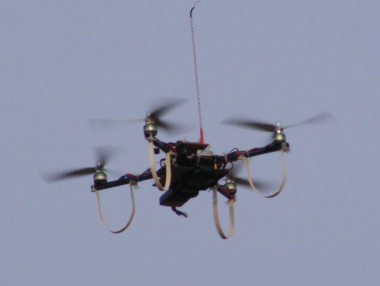
\includegraphics[width=0.5\textwidth]{quadrotor.jpg}
    \caption{Picture of a quad-rotor flying.}
\end{figure}

Further, the autonomous quadrotor system is used to carry payloads. The dynamics for the system becomes really complex due to the presence of joints and their interactions with the system. The joints may be rigid or non-rigid. The problem here changes from controlling the motion of the quadrotor to controlling the motion of the payload. 

Another idea explored is to use a similar abstraction of the system such that the system changes minimally with change in external parameters such as wind, external payload etc. and also for re-using or transferring the knowledge that is acquired in this case. 

\section{Project description}
The project's goals can be summarised as follows:
\begin{itemize}
	\item {Low level Quadrotor control: This can be explained as reaching a state from the current state. It is termed as low level control since we have imparted to the system no knowledge of what model the system should follow, and it directly interacts with the hardware of the system. It acts in order to ensure that the stability of the system is maintained as well.}
	\item {High level control or Trajectory tracking: Here, the system actually uses the low level controller that is learnt using Reinforcement Learning, and on top of that implements a control system to achieve a trajectory in the best possible way.}
	\item {Further, we explored adding a payload to the system coupled with a set of one or more joints. Here the focus shifted from using a controller for achieving a certain quadrotor trajectory or position, to doing the same for the payload. This becomes an interesting application commercially as well.}
	\item {Apprenticeship based learning: In cases where specifying the system's trajectory is complicated, but it is easy for an expert to perform the same, we employ Apprenticeship based learning. The aim is to learn through observing an expert's multiple demonstrations and finding the optimal control for the same.}
\end{itemize}

\chapter{Background}
\section {The Reinforcement Learning problem}
Reinforcement Learning is the computational approach of learning from interaction. The problem is defined as a closed-loop problem where the actions taken by the learner influence its later inputs. The learner(agent) has to discover which actions achieve the highest payoffs(reward) with its interaction with the environment. 

The rewards considered might not be the immediate rewards but also include subsequent rewards. A simple example of Reinforcement Learning would be how babies learn to walk. Their action influences how well they would be able to walk further, and rewards are received in this case, say for example as a punishment that would be falling. It is essential to note that as mentioned above, the reward received might not correspond to the immediate action, but to wrong actions taken in the past during the course of walking. Some of the fundamentals and nomenclature in the field of Reinforcement Learning are as follows:
\begin{itemize}
\item{Agent: The learner represents the agent, and has the capability of taking actions from a given action space $A$}
\item{State: The state is the representation of the agent on the basis of which an action is taken. It is represented by a State space $S$}
\item{Policy: It represents the learner's way of taking an action based on the perceived state of the environment. The policy may be represented as a simple lookup table or some function approximation in most of the cases. Policies may be stochastic in nature.
The policy can be represented by: $\pi: S\rightarrow A$}

\item{Reward signal defines the goal of a reinforcement learning problem. It is a way of communicating to the learner/agent, about how good the action taken by the agent is. The agent has the capability to alter the reward only through its action taken. The agent always tries to maximize the reward received in the long run.}
\item{Value function specifies how good the rewards are in the long run. Value of a state is represented as the expectation of the total reward that the agent accumulates from the starting state.  $V^{\pi} (s) = E[R|s,\pi]$}
\end{itemize}

\begin{figure}[H]
  \centering
    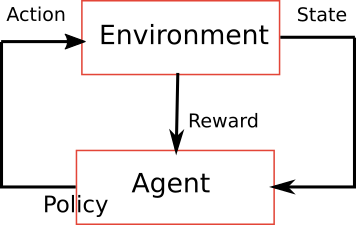
\includegraphics[width=0.6\textwidth]{RL.png}
    \caption{Representation of RL system}
\end{figure}

\section {Markov Decision Process}
A Markov Decision Process (MDP) is based on a Markov Chain ie only the current state influences the next state. The transition matrix depends on the action taken by the decision maker (agent) at each time step. The determining feature of a Markov chain is that:
\begin{equation}
\Pr(X_{n+1}=x\mid X_1=x_1, X_2=x_2, \ldots, X_n=x_n) = \Pr(X_{n+1}=x\mid X_n=x_n)
\end{equation}
A Markov decision process is represented by a tuple:
\begin{equation}
[S, A, P_a(s,s'), R_a(s,s'), \gamma]
\end{equation}
where\\
$S$ is a finite set of states,\\
$A$ is a finite set of actions,\\
$P_a(s,s') = \Pr(s_{t+1}=s' \mid s_t=s, a_t=a)$ is the probability that action $a$ in state $s$ at time $t$ will lead to state $s'$ at time $t+1$,\\
$R_a(s,s')$ is the immediate reward (or expected immediate reward) received after transition to state $s'$ from state $s$, and\\
$\gamma \in [0,1]$ is the discount factor, which represents the difference in importance between future rewards and present rewards.

%\section{Continuous states and actions}
%A dynamic control like quadrotor control comprises of continuous states and actions. Many existing Reinforcement Learning techniques assume discrete sets for states and actions, due to which, continuous variables need to be discretized. 
%
%A more reasonable approach is to use function approximation. Function approximation provides an elegant solution to multi-dimensional spaces. And in most cases, using a function approximation reduces the space to a smaller subspace. And optimality conditions within this subspace still hold true. Hence, to achieve an optimal solution, even function approximation needs to be carried out carefully.
%
%In policy search methods, the policy function is directly function approximated. In such cases, the policies that are searched (the policy class or policy family) are restricted due to this parametrization. If the function approximation and parametrization is not done correctly, the optimal policy may not be part of the policy class. In such cases, the result got from a typical policy search algorithm is simply the optimal solution in this subspace defined by the policy class.


\section{Quadrotor dynamics}
Quadrotors are complex systems with respect to dynamics and control. Haivng six degrees of freedom (three translational and three rotational) and only four independent inputs (rotor speeds), quadrotors are severely underactuated. The quadrotor motors are used to control the altitude, pitch, roll, and yaw of the quadrotor, which in turn can represent the 6 degree motion of the system.
\begin{figure}[H]
  \centering
    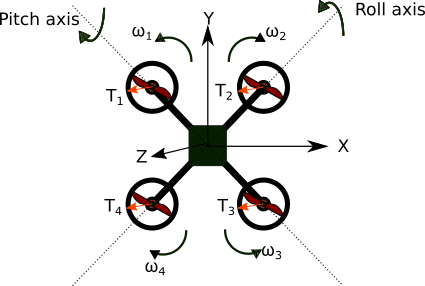
\includegraphics[width=0.7\textwidth]{Quadrotor_fbd.png}
    \caption{Free body diagram of quadrotor}
\end{figure}
Combining the revolutions per minute (rpm) of the 4 rotors makes it possible for the quad-rotor to turn, and move in various ways. Quadrotor motion can be achieved in 2 configurations: "X" and "+" configurations. Both the quadrotor configurations are nearly identical with differences in controlling the quadrotor. The X configuration proves to be better in terms of stability and faster response to the control system. Hence, we have used X configuration for our system, and will be discussing control for the same.

\subsection*{Quadrotor motion}
Quadrotor motion can be analyzed by considering 3 independent motions. Although, all these motions have interdependent controls, an understanding can be reached for the control needed for the quadrotor.

{\bf Altitude (z)}: To change altitude (in the positive z direction), equal thrust is applied to all the rotors. The moment of the quadrotor is balanced by giving equal thrusts to opposite motors but having 2 motors spin in 1 direction, and other 2 in the opposite one. The same principles hold during hovering of the quadrotor.
\begin{figure}[H]
  \centering
    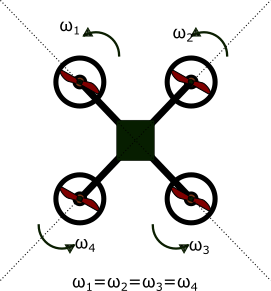
\includegraphics[width=0.5\textwidth]{Quadrotor_altitude.png}
    \caption{The configuration of the 4 rotors of a quad-rotor to change altitude.}
\end{figure}

{\bf Yaw}: For changing the yaw, the thrust is applied to the rotors causing an unbalanced moment. It is done by increasing speed of one pair of opposite rotors and decreasing speed of the other pair by the same amount. Thus the total thrust on the quadrotor remains constant and the only motion occuring is the yaw motion.
\begin{figure}[H]
  \centering
    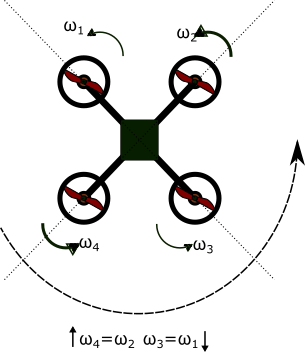
\includegraphics[width=0.5\textwidth]{Quadrotor_yaw.png}
    \caption{The configuration of the 4 rotors of a quad-rotor to change yaw.}
\end{figure}

{\bf Pitch and Roll}: For pitch and roll, the opposite pair of motors responsible for maintaining the stability of the quadrotor have to change velocities. One of the thrusts is reduced while the other one is increased which causes the quadrotor to move in a certain direction. Both pitch and roll motions are completely identical by symmetry.
\begin{figure}[H]
  \centering
    \begin{subfigure}[c]{0.45\textwidth}
      \centering
        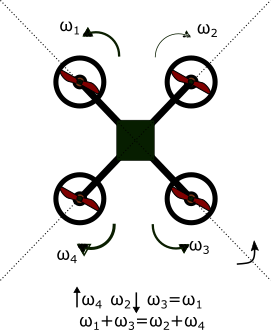
\includegraphics[width=\textwidth]{Quadrotor_roll.png}
        \caption{}
    \end{subfigure}
    \quad
    \begin{subfigure}[c]{0.45\textwidth}
      \centering
        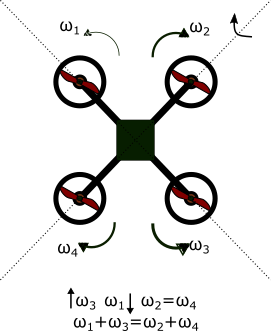
\includegraphics[width=\textwidth]{Quadrotor_pitch.png}
        \caption{}
    \end{subfigure}
    \caption{The configuration of the 4 rotors of a quad-rotor to change roll and pitch.}
\end{figure}

\subsection*{Dynamics model}
The quadrotor dynamics have been documented by Samir Bouabdallah and Roland Siegwart for the OS4 project \cite{QuadrotorDynamics}. This modelling is used in the Hector Quadrotor package. The paper involves modelling of each of the parts separately starting from modelling of the motors, followed by modelling aerodynamics of the complete system. In addition the hub forces, drag moment and rolling moment are found for the quadrotor to find the total forces on the quadrotor. Finally, the transition function arrived at is given by:
\begin{equation} \begin{split}
  f(\bar{S}, \bar{U}) = \left\{
    \begin{array}{c}
      \dot{\phi} \\
      \dot{\theta} \dot{\psi} a_{1} + \dot{\theta} a_{2} \omega_{r} + b_{1} U_{2} \\
      \dot{\theta} \\
      \dot{\phi} \dot{\psi} a_{1} + \dot{\phi} a_{4} \omega_{r} + b_{2} U_{3} \\
      \dot{\psi} \\
      \dot{\theta} \dot{\phi} a_{5} + b_{3} U_{4} \\
      \dot{z} \\
      g  - (\cos{\phi} \cos{\theta})\frac{U_{1}}{m} \\
      \dot{x} \\
      u_{x} \frac{U_{1}}{m} \\
      \dot{y} \\
      u_{y} \frac{U_{1}}{m}
    \end{array}
  \right\}
\end{split} \end{equation}
where $\bar{U}$ is the action, the constants $m$, $a_{i}$, and $b_{i}$ are system parameters that can be calculated from properties like moment of inertia, mass, etc. $u_{j}$ is the projection from Spherical co-ordinates to Cartesian of a unit vector in the $j$ dimension in Cartesian co-ordinates.


\chapter{Literature review}
Reinforcement learning has been successful in all sorts of applications like marketing strategy selection and advertisement targeting, cell-phone network routing and multiplexing, bipedal to octopedal locomotion, and efficient web-page indexing.
Reinforcement learning has been applied to a wide variety of spheres ranging from robotics \cite{HelicopterPegasus} to game playing like checkers \cite{RLInCheckers}, the game of Go \cite{RLInGo} and the famous TD-Gammon player \cite{RLInBackgammon}. The game agents were able to beat some of the best players of the time. The gaming agents led to advancements in the theory of backgammon and recently may do the same in Go as it explores strategies humans have not experimented with. Reinforcement Learning has also been applied to routing (Q-routing) \cite{RLInQRouting},
improving elevator dispatch performance \cite{RLInElevators}, algorithm selection \cite{RLInAlgoSelection}, job-shop scheduling \cite{RLInJobShopScheduling}, dialog systems \cite{RLInDialogSystems}, maze solving with multi agents \cite{PredatorPrey}, and recommendation systems \cite{RLInRecommenders}.

\section{Reinforcement learning in control}
Reinforcement learning has been applied to control problems frequently such as table tennis\cite{TableTennisRL}, Soccer playing bots\cite{RobocupRL}, Helicopter control\cite{HelicopterPegasus} etc. RL has been used a lot in control systems application as it is very closely related to the theory of classical optimal control, as well as dynamic programming, stochastic programming, simulation-optimization, stochastic search, and optimal stopping. RL addresses the problem of finding the optimal policy for optimizing an objective function and both have similar notions of states, actions and transitions.

The review \cite{ControlForQuads} by Andrew Zulu and Samuel John gives an overview of techniques that have been used for Autonomous Quadrotor control. It speaks of techniques that merge control theory and machine learning. Fuzzy logic based controls to fuzzify control theory algorithms are frequently used. For example, Fuzzy logic to identify the constants required in PID and LQR were researched by E. Abbasi and J. Mahjoob.

One of the most important approaches to reinforcement learning is the use of classical optimal control techniques (e.g. Linear-Quadratic Regulation and Differential Dynamic Programming) to system models learned via repeated interaction with the environment, for example \cite{NonparametricRL} and \cite{HelicopterPolicySearch}. Reinforcement learning is often viewed as "adaptive optimal control".  In fact, many of the methods thus far demonstrated on difficult problems have been model-based systems that are derived from control theory for example, \cite{LWL} and \cite{PILCO}.
 
\section{Payload control for UAVs}
There has been some work to control the payload of an UAV directly using Control Theory \cite{PayloadControlTheory,PayloadControlTheory2}. These approaches require the complete knowledge of the system dynamics.  

There has also been some work in controlling payloads of UAVs using Reinforcement Learning \cite{PayloadLSPI}. In this, Least Square Policy Iteration (LSPI) is used. Three different LSPI are used to track the x, y, and z dimensions. This has the disadvantage of these three learning policy iterations that can clash with each other.

\section{Pure Pursuit}
Pure pursuit\cite{PurePursuit} is a tracking algorithm that works by calculating the curvature that will move a vehicle from its current position to some goal position. The name pure pursuit comes from the analogy of driving a vehicle chasing a certain distance ahead of it, coming from the way humans drive. For wheeled vehicles, the curvature of the motion also needs to be calculated for moving back to the trajectory due to the fact that the drive is non-holonomic, ie moving left is much different from moving front due to the turn radius involved.

\subsection*{Effect of lookahead distance}
The parameter for the algorithm is the lookahead distance for the system which decides how aggressively the system should try getting back onto the desired trajectory. A shorter lookahead would cause the system to be closer to the trajectory, but the unstability might be higher due to overshooting, and a longer lookahead would cause the system to be much more stable in following the trajectory, and would be able to reach the trajectory much more slowly.

\begin{figure}[H]
  \centering
    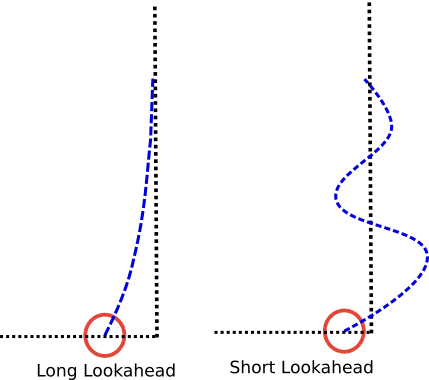
\includegraphics[width=0.5\textwidth]{Pure_Pursuit_path.png}
    \caption{The figure shows the impact of different lookahead distances on the trajectory considering a holonomic system.}
\end{figure}


\section{PEGASUS}
PEGASUS \cite{PEGASUS} (Policy Evaluation-of-Goodness And Search Using Scenarios) is a direct policy search method by using a deterministic simulative model of the system, ie the stochasticity of the system doesn't come from the system itself. It is a policy gradient method which has been extended to continuous state and action spaces.

\subsection*{Definitions}
\subsubsection{Partially observable Markov Decision Process(POMDP)}
POMDPs are generalizations of MDPs where it is assumed that the agent can't observe the complete underlying state, however the system behaviour is Markov chain. It is can be viewed as a much more closer indicator to real world as compared to Markov systems.

\subsubsection{Value of the policy}
Value of a policy is similar to value to a state from Reinforcement learning and can be used to compare different policies. The value of the policy is given as the expected value of the initial state in an episode. Since the system a) can have different initial states, and b) is stochastic, we need to consider multiple observations of the system to estimate the value of the policy.
\begin{equation}
  V(\pi) = \mathbf{E}_{s_{0} \sim \mathbb{D}} [ V^{\pi} (s_{0})]
\end{equation}

%%%%%%%%%%%%%%%%%%%%%%%%%%%%%%%%%%%%%%%%%%%%%%%%%%%%%%%%%%%%%%%%%%%%%%%%%%%%%%%%%%%%%%%%%%%%%%%%%%%%%%%%%%%%%%%%%%%%%%%%%%%%%%%%%%%%%%%%
\subsection*{Transformation of POMDP}
Given a (PO)MDP $M$ and a policy class, a transformed POMDP $M'$ and a corresponding policy class is constructed to make the transitions deterministic using a deterministic simulated model $g$. The transformed state $s$ in $M'$ is represented by
\begin{equation}
	\bar{s} = (s, p_1, p_2, p_3......)
\end{equation}
On taking an action $a$ in state $\bar{s}$, the transition is to a state $\bar{s}'$ represented by
\begin{equation}
	\bar{s}' = g(\bar{s}, a, p_2, p_3, ....) 
\end{equation}
The vector $p(p_1, p_2, p_3 ....)$ is sampled randomly as $[0,1]^{\infty}$ and is used to represent all the stochasticity in the transition functions in the system. The same distribution $p$ is used running each Monte-carlo  simulations, and hence the model is deterministic simulated. The initial state is chosen according to a uniform distribution and the Policy and the reward function are transformed according to the new MDP as $\bar{R}(\bar{s}, a) = R(s, a)$ and $\bar{\pi}(\bar{s}) = \pi(s)$.

The equivalence of the transformed MDP is proved by proving that $V_M(\pi)=V_{M'}(\bar{\pi})$ which means that the deterministic simulative model can be used in place of the original MDP.
		
%%%%%%%%%%%%%%%%%%%%%%%%%%%%%%%%%%%%%%%%%%%%%%%%%%%%%%%%%%%%%%%%%%%%%%%%%%%%%%%%%%%%%%%%%%%%%%%%%%%%%%%%%%%%%%%%%%%%%%%%%%%%%%%%%%%%%%%%%%%%%%%%%%%%%%%%%%%%%%%%%%%%%%%%%%%%%%%%%%%%%%%%%%%%%%%%

\subsection*{Obtaining optimal policy}
The optimality of the policy is compared using the value of the policy. Since a transformed POMDP can be used in place of the original one, we find the policy for the transformed POMDP. The value for a policy is approximated by replacing the expectation by the mean of a finite samples ie 
\begin{equation}
	V_{M'}({\pi}) \approx  \frac{1}{m} \sum_{i=1}^{m} V_{M'}^\pi(s_o^{(i)})
\end{equation}
This can be written as the average of returns given during each of the runs:
\begin{equation}
	V_{M'}({\pi}) = \frac{1}{m} \sum_{i=1}^{m} \{\bar{R}(s_0^{(i)})+\gamma \bar{R}(s_1^{(i)}) + ..... + \gamma^H \bar{R}(s_H^{(i)}) \}
\end{equation}
where m represents the initial states sampled for which the rewards were collected and H is the horizon time, ie the number of steps after which the expected error is less than some threshold. The xinitial state ($s_0$) is sampled from the distribution of initial states ($\mathbb{D}$). 

The optimal policy is defined as the one with the maximum value for the policy, ie
\begin{equation}
  \pi^{*} = {\arg \max}_{\pi \forall \mathbf{\Pi}} {V_M(\pi)}
\end{equation}

\subsection*{Discrete vs Continuous state action spaces}
In a problem where the actions are discrete and an episode terminates after a fixed number of steps, a policy can be found easily using the above equation. In case the episode doesn't have a termination step, the Horizon time parameter can be set such as to get a value of the policy. The optimal policy would be the one with the maximum value of the policy.

However, in a problem where actions are continuous, the policy needs to be generalized using a function approximation. Additionally, finding all the policies and comparing them isn't feasible. In this case, the policy's class is assumed as a parameteric set of functions, and can be solved using a maximization technique such as gradient descent, stochastic gradient descent, etc. The policies obtained using this method $\pi_{\theta}$, are the projections of the optimal policy on the policy class $\pi$ with $V(\pi)=V(\pi_{\theta})$ where $\theta$ represents the parameters for the policy class.

\begin{figure}[H]
  \centering
    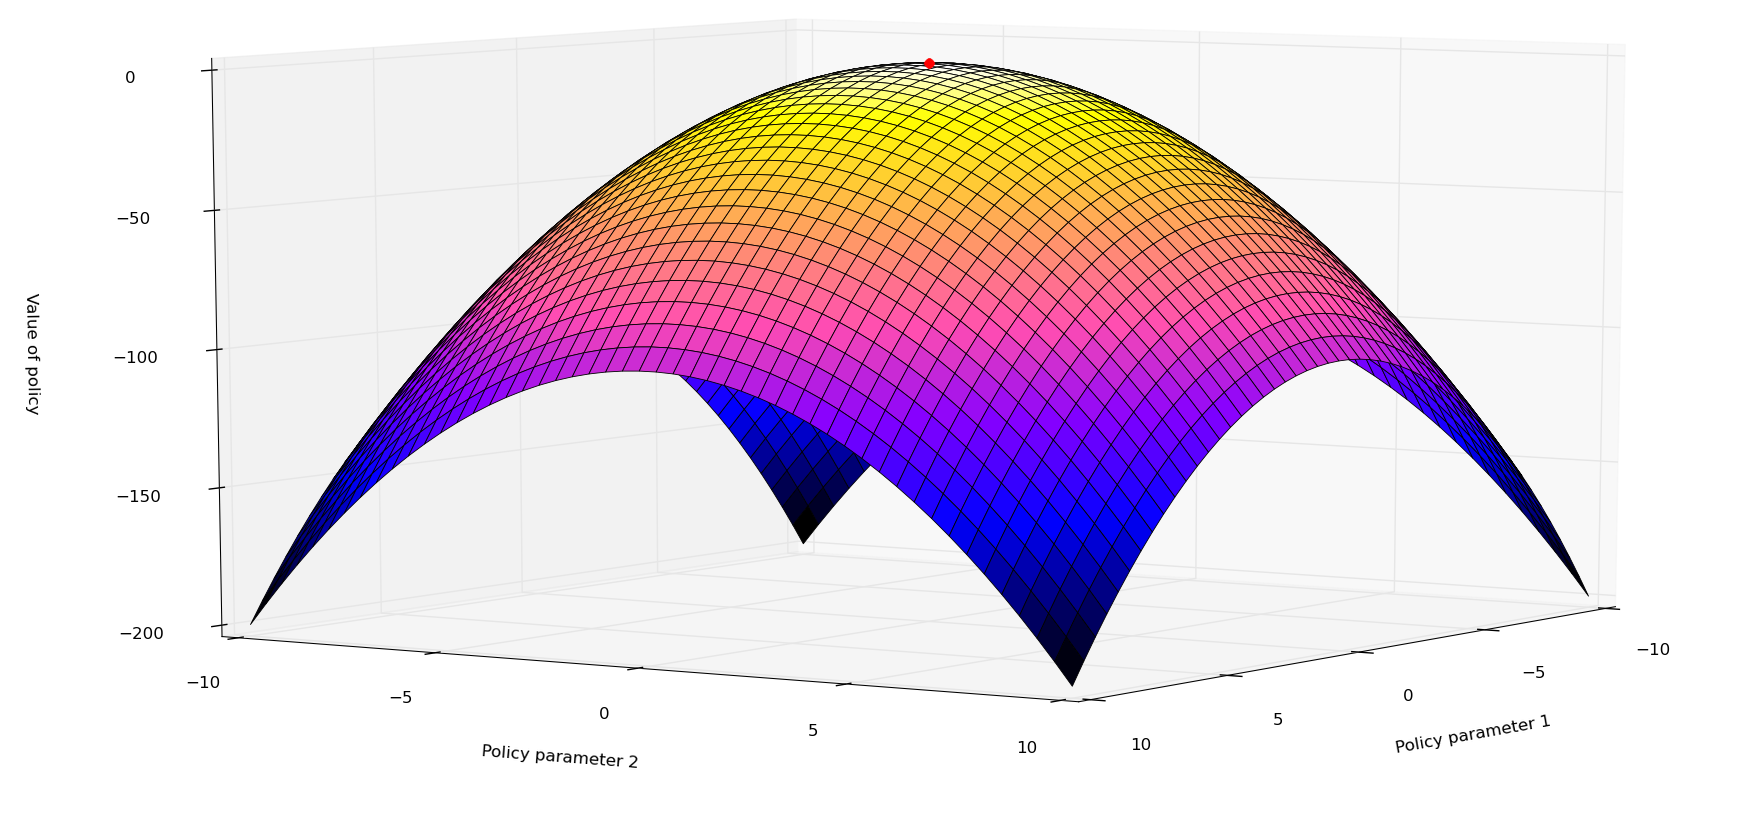
\includegraphics[width=\textwidth]{gradient_descent.png}
    \caption{Two parameter policy. The value of the optimal policy can be found using a maximization technique.}
\end{figure}

\subsection*{Application to helicopters}

PEGASUS has already been used in helicopters \cite{HelicopterPegasus}. In their paper they describe using PEGASUS on a model they created of the helicopter. The learning happened on the model and the policy learnt was implemented on the actual helicopter and obtained successful results.

The policy class was used as a neural network with the weights as parameters of the policy to be learnt as PEGASUS. This method although provides a much easier way to learn the model without having much knowledge of the system, overfits the given system and trying to understand the system physically can be a hard task.
The reward function used is the L2 norm of the difference between the expected position and the original position. It includes the x, y, z position as well as the yaw. An additional negative reward is added to discourage behaviour like jerky accelerations, fast motion etc. With this system, they were able to make the quad-rotor hover and move in l	ines successfully.

\begin{figure}[H]
  \centering
    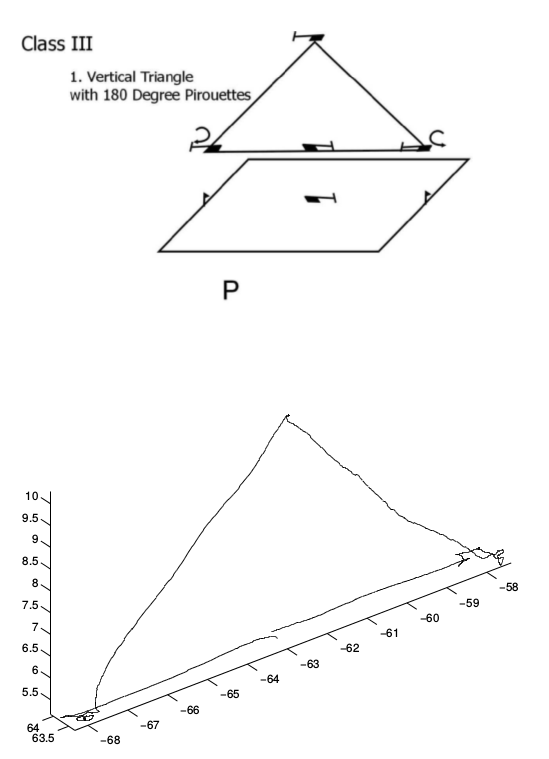
\includegraphics[width=0.4\textwidth]{pegasus_helicopter.png}
    \caption{Control of a helicopter using PEGASUS by Andrew Ng, Jin Kim, Michael Jordan and Shankar Sastry \cite{HelicopterPegasus}. A comparison of maneuver diagrams from RC helicopter competition\protect\footnotemark \space compared with actual trajectories from the model learnt by PEGASUS.}
\end{figure}
\footnotetext{Maneuver diagrams taken from http://www.modelaircraft.org}

\subsection*{Quadrotor Aerobatics}
There has been some later work on using PEGASUS along with Apprenticeship learning in helicopters to do complex tasks like aerobatics \cite{ApprenticeshipHelicopterAerobatics}. Apprenticeship learning provides an efficient method to create a reward function, and PEGASUS learns the policy based on the generated reward function.

Additionally, there has also been work on using PEGASUS for outright unstable states that are difficult for most human pilots. The work by Andrew Ng, Jin Kim, Michael Jordan and Shankar Sastry on Inverted helicopter flight \cite{InvertedHelicopterFlight} uses PEGASUS with an underlying controller. The underlying controller provides a flexibility to the system and generalizes it further.

\begin{figure}[H]
  \centering
    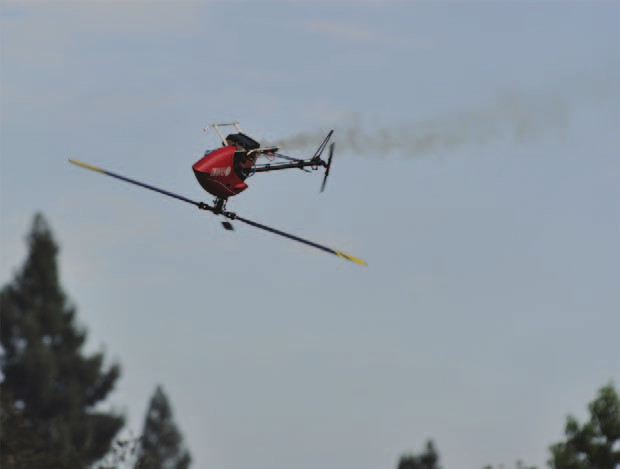
\includegraphics[width=0.5\textwidth]{pegasus_inverted_helicopter.png}
    \caption{Control of a helicopter to hover inverted using Apprenticeship Learning and PEGASUS by Andrew Ng, Jin Kim, Michael Jordan and Shankar Sastry \cite{InvertedHelicopterFlight}.}
\end{figure}

\section{Apprenticeship Learning}
Some of the problems faced in reinforcement learning are: 
\begin{itemize}
	\item Unavailability of a closed form or formal specification of the control task or defining the problem to be learnt. One example could be the quality of flight for a system. 
	\item For real world systems, the dynamics become very complicated and hard to model due to the high dimensionality and stochasticity.
\end{itemize}
Apprenticeship learning tries to solve the above problems, by reducing the dependence of the conventional reward function in reinforcement learning. The aim is to learn the task to be done without really providing a mathematical representation of the same. It was introduced by Peter Abeel\cite{ApprenticeshipLearningThesis} 

\subsection{Inverse Reinforcement Learning}
Inverse Reinforcement Learning\cite{InverseRL} (IRL) is a field of Reinforcement learning where the agent tries to learn the reward function by analyzing observations of an expert. It is proved that  the rewards learnt by the agent, although would not be the same as the expert's reward function, the agent is able to achieve the optimal policy.
\begin{equation}
E_{s_0 \sim D}[V^\pi(s_0)] = w^T \mu(\pi)
\end{equation}
where $w$ represents the represents the assumed reward structure and $\mu$ is the feature expectations of the policy. 

\subsubsection*{Optimality of the learnt policy}
It is proved that if we find a sufficiently good policy such that $\mu(\pi)-\mu*<\epsilon$, then for any reward structure $w$, the expected value of the policy would be within $epsilon$. The algorithm runs by doing an iterative computation by finding the policy and the rewards, since the optimal policy is unknown and terminates when the error in feature expectations is sufficiently low.

\subsubsection*{Application in driving}
Inverse RL based systems were employed for implementing a car-driving simulation game, where apprenticeship learning was tried to learn different driving styles. Here, the reward is dependent on how the expert drives the car, and the system was able to mimic the same.

Additionally, the system was implemented to do path planning for parking by the Stanford racing team in the DARPA Urban Challenge\cite{ApprenticeshipDARPA}. The system's sensor data was collected as the driver was asked to park the vehicle in 3 different driving styles.
\begin{figure}[H]
  \centering
  \begin{subfigure}[t]{\textwidth}
    \centering
      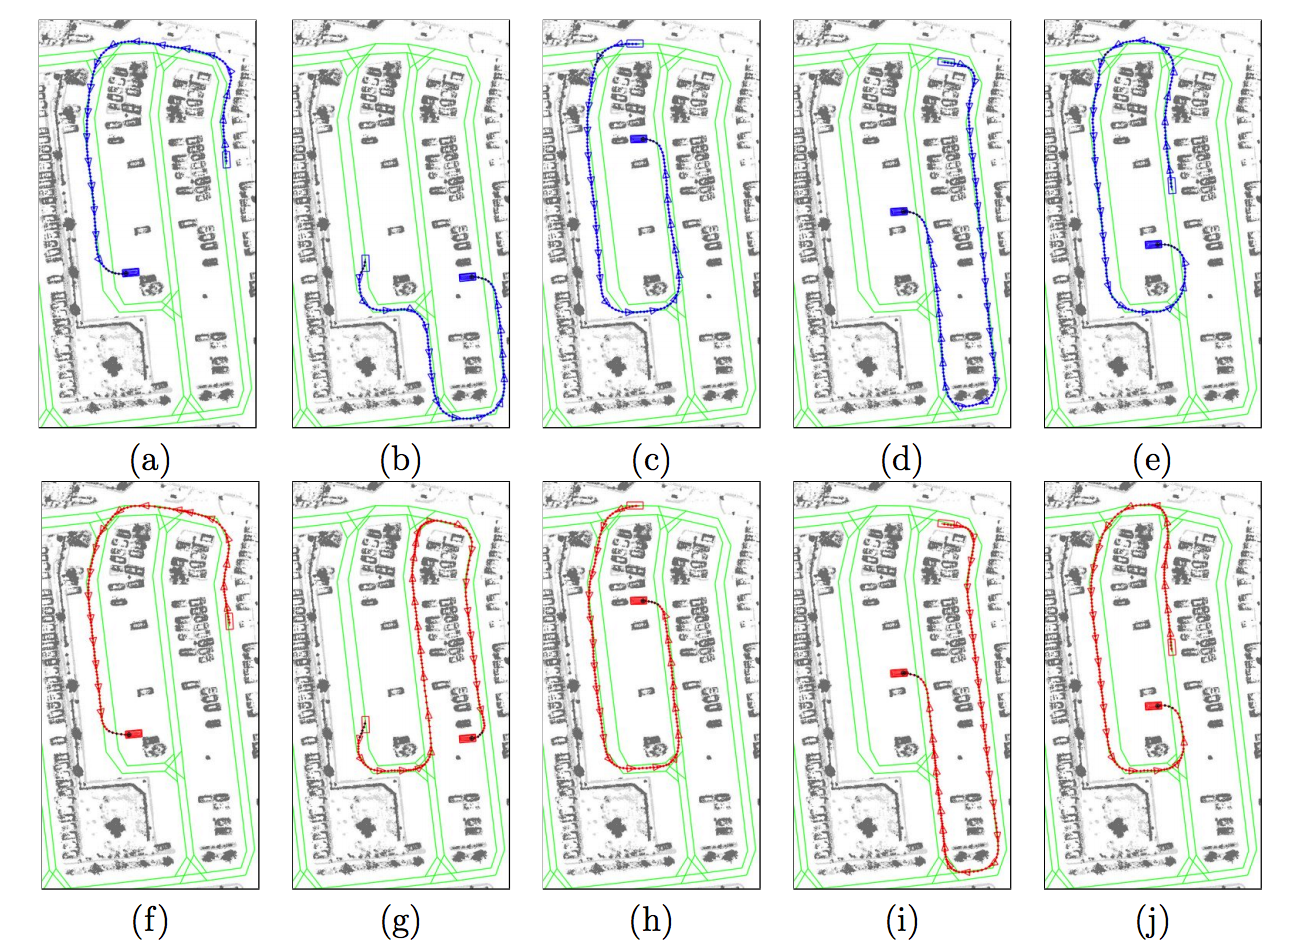
\includegraphics[width=\textwidth]{IRL_nice.png}
      \caption{"Nice" parking style}
  \end{subfigure}
  \quad
  \begin{subfigure}[t]{\textwidth}
    \centering
      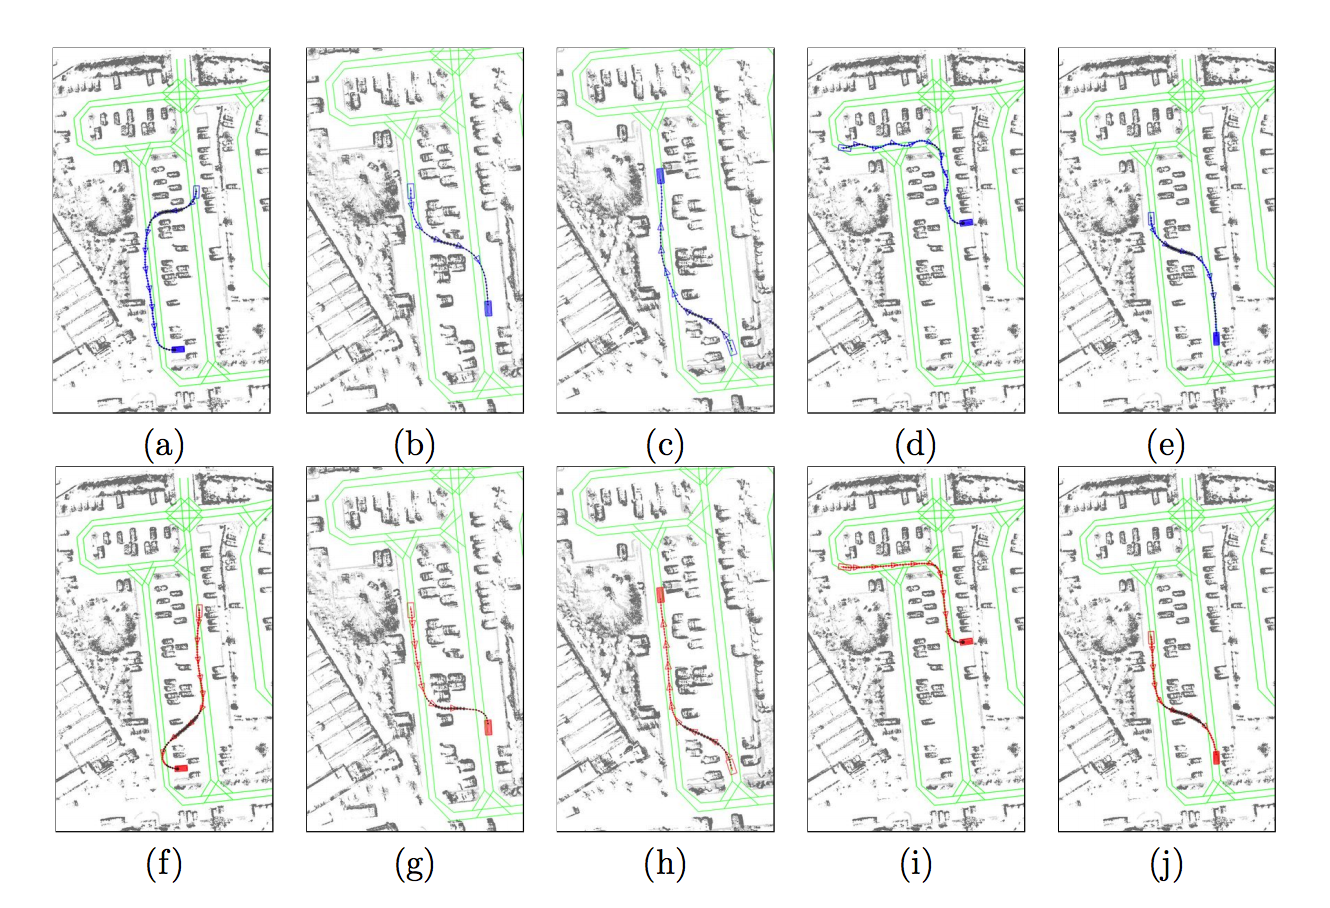
\includegraphics[width=\textwidth]{IRL_sloppy.png}
      \caption{"Sloppy" parking style}
  \end{subfigure}
  \caption{Comparison of different parking styles learnt and performed using inverse RL. In each figure, (a) to (e) represent the expert and (f) to (g) represent the agent trying to mimic the style.}
\end{figure}

%%%%%%%%%%%%%%%%%%%%%%%%%%%%%%%%%%%%%%%%%%%%%%%%%%%%%%%%%%%%%%%%%%%%%%
\subsection*{Dynamic Time Warping}

Dynamic time warping is an algorithm that measures similarity between two temporal sequences which vary in time or speed. It is well known for application in speech recognition\cite{DTW} to work with different speaking speeds. It It calculates an optimal match between two time series with the following constraints: a) Monotonicity b) Continuity condition and c) Boundary condition.

Additional constraints can be added to remove error conditions, such as: Window conditions and slope conditions restricting the warped sequence to close to the diagonal.
\begin{figure}[H]
  \centering
  \begin{subfigure}[t]{0.7\textwidth}
    \centering
      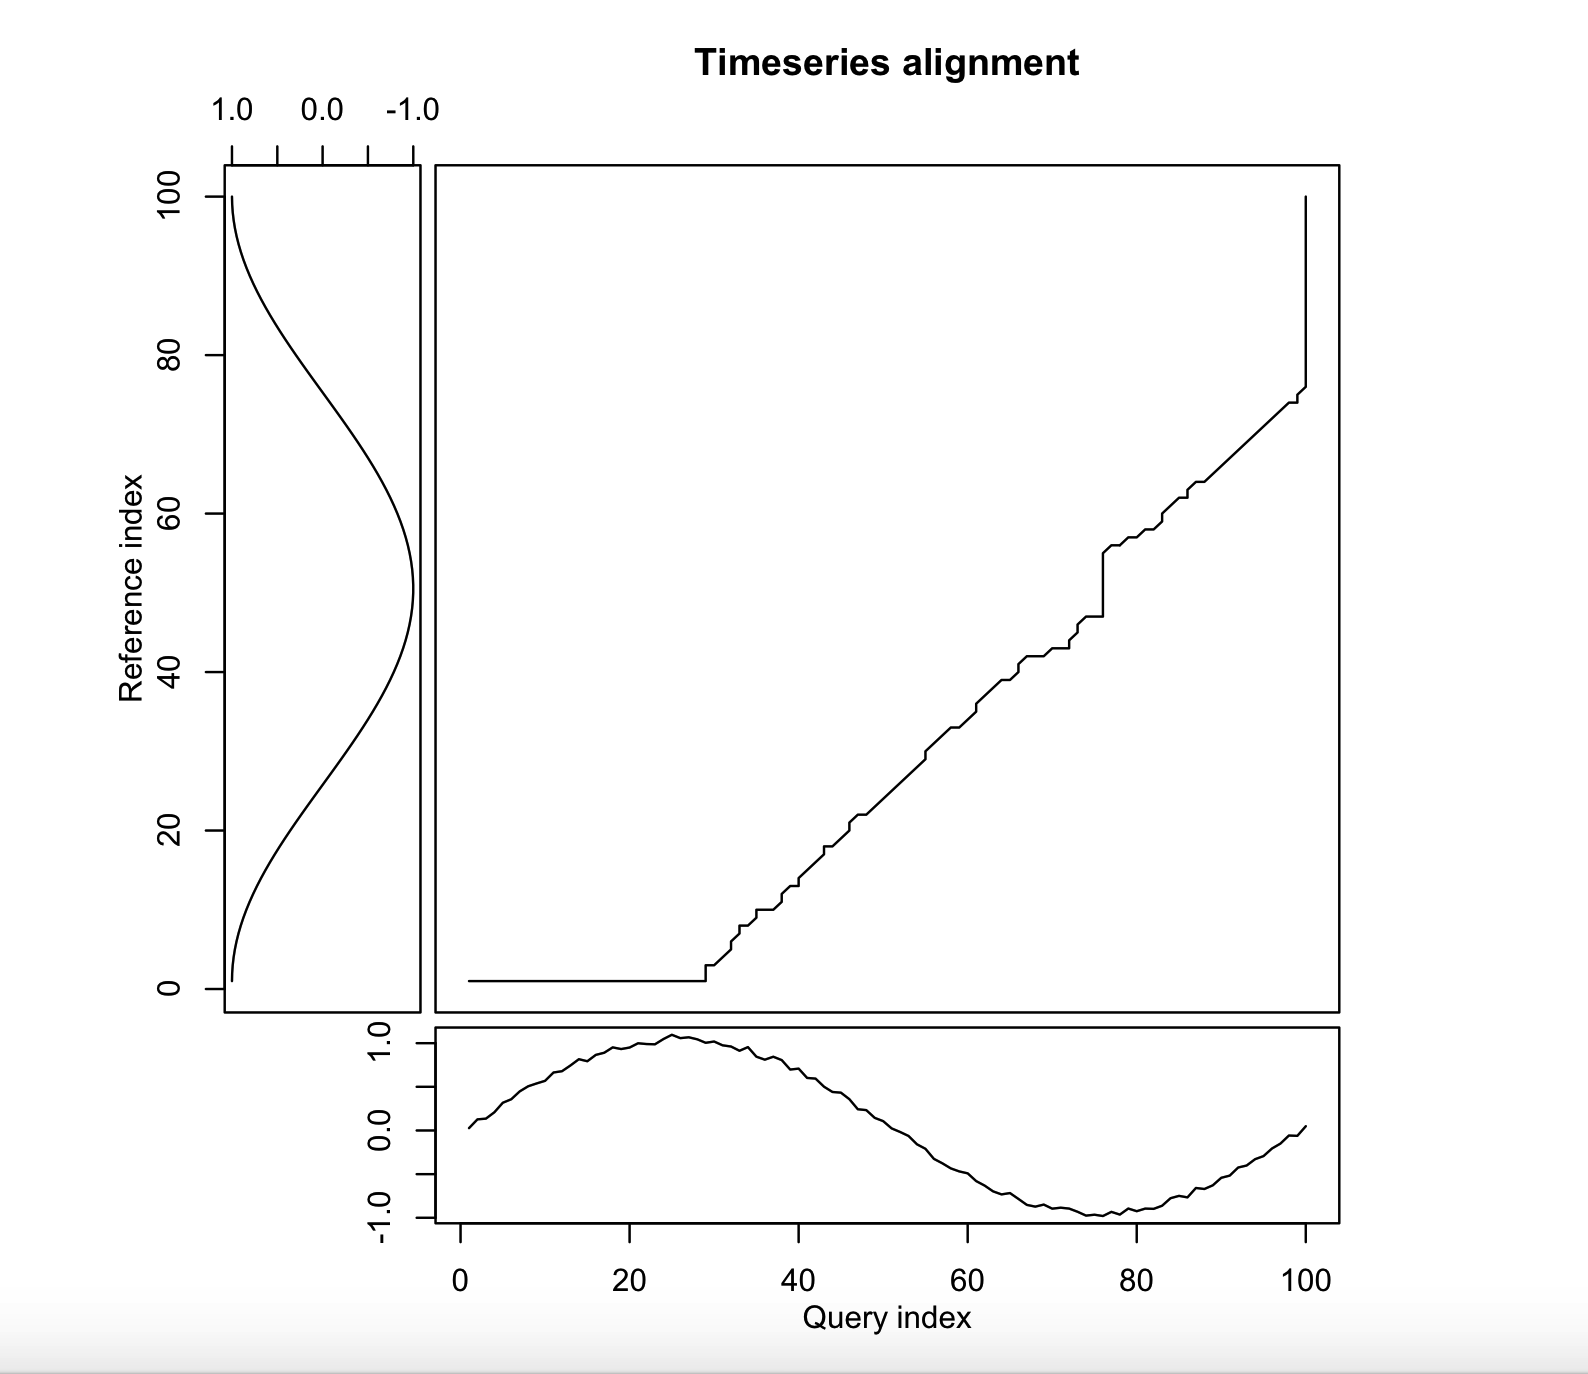
\includegraphics[width=\textwidth]{DTW.png}
  \end{subfigure}
  \quad
  \begin{subfigure}[t]{0.7\textwidth}
    \centering
      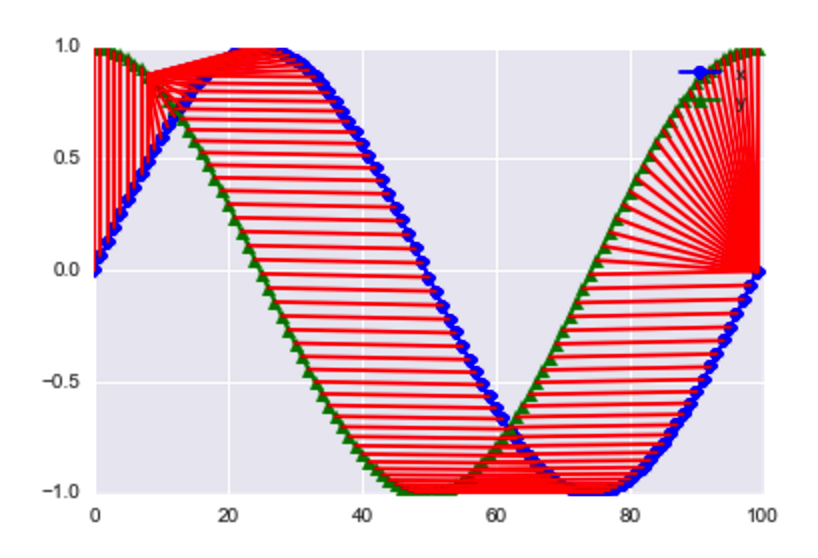
\includegraphics[width=\textwidth]{DTW2.png}
  \end{subfigure}
  \caption{Dynamic time warping to compare 2 shifted signals.}
\end{figure}

\subsubsection{Windowing}
The optimal result provided by DTW can be wrong at times, where the warped time dimensions are too far. This means that the warping is too severe ie the two sequences aren't comparable. This can be solved by windowing the output of DTW to a region around the diagonal. Multiple windowing techniques can be used for the same. Some of the popular ones are: itakura windowing, sakoechiba windowing, and slanted-band windowing which are implemented in the R "dtw" package \cite{RDTWPackage}. 

\subsection*{Extended Kalman Smoothing for non-linear dynamical systems}
Kalman filters \cite{KalmanFilters} also known as Linear Quadratic Estimation (LQE) are used concepts in time series and control systems. It is an algorithm to use a series of models with expected errors for measurements and use it to estimate hidden variables. One use of the same is predicting states for a system\cite{KalmanFiltersFusion} like a quadrotor by "fusing" inputs from different sensors like IMU, camera, LIDAR etc. It can easily be used to predict the model for the system and filter out erroneous readings from sensors. A Kalman filter can be used for filtering, smoothening, and predicting states for a system.

An extended Kalman filter\cite{NonLinearEMKalman} can be used to extend the Kalman filter based model to a non-linear dynamics case such as a quadrotor system.  

%%%%%%%%%%%%%%%%%%%%%%%%%%%%%%%%%%%%%%%%%%%%%%%%%%%%%%%%%%%%
\subsection{Learning trajectories from multiple demonstrations}
Following a desired trajectory using a complex non-linear model is a hard task. It requires to specify the trajectory mathematically, and at the same time have compatibility with the quadrotor dynamics system. In such a system, if an expert is available, it becomes much more easier to learn the trajectory by having the agent observe the expert controlling\cite{ApprenticeshipHelicopterAerobatics} the trajectory, and incorporate some additional known information about the trajectory known by the system.

\subsubsection {Learning the model}
The model required for this system can be an approximate one\cite{InaccurateRLmodels}, and hence is found by first obtaining lot of flight data for the system, and then fitting it into an approximate model for the system. This is used only as a baseline model for the trajectory.

\subsubsection{Generative model}
The trajectory collected from observations is assumed to be sub-optimal due to being controlled by a human. The system tries to estimate the actual trajectory by assuming a Gaussian model for the observations and the non-linear dynamics of the helicopter and estimate an optimal trajectory by the same. The basic generative model for the system is assumed as:
\begin{equation}
  x_{t+1} = f_{t} (x_{t}) + {\omega}_{t}^{(x)}, \qquad \omega_t^{(x)} \sim \mathcal{N} (0, \Sigma^{(x)})
\end{equation}
where $x_t$ represents the hidden state of the system at time $t$. The demonstrated trajectories are assumed to map to the hidden trajectory using a Normal distribution.
\begin{equation}
  y_{t}^{k} = h(x_{\tau_t^k}) + {\omega}_{t}^{(y)}, \qquad \omega_t^{(y)} \sim \mathcal{N} (0, \Sigma^{(y)})
\end{equation}

\subsubsection{Obtaining hidden trajectory}
The hidden trajectory is found using $M$ different demonstrated trajectories given by the expert with time steps $N^k$. The observed trajectory is represented as collection of states and actions. 
\begin{equation}
	\begin{array}{c}
	y_j^k = \left(\begin{array}{c}
		s_j^k\\
		u_j^k
	\end{array}\right) \forall j=0..N^k-1, k=0..M-1\\
	z_t = \left(\begin{array}{c}
		s^*_t\\
		u^*_t
	\end{array}\right) \forall t=0..T-1
	\end{array}
\end{equation}
where $y$ represents the observed trajectories with states $s$ and actions $u$ and $z$ represents the optimal hidden trajectory.


\subsubsection*{Matching time series for observations}
For different series of observations, we intend to find $\tau_t^k$, ie  the time step in the intended trajectory mapped to the observed trajectory at time step $t$. The total time steps in the hidden trajectory is taken as twice the average of the demonstrations:
\begin{equation}
  T = 2 \left( \frac{1}{M} \sum_{k=1}^{M} N^k \right)
\end{equation}

The different observations are compared using the DTW\cite{DTW} algorithm, since each of the observed states can be at a different time step.


\subsubsection*{Trajectory Estimation}
In the quadrotor aerobatics paper, \cite{ApprenticeshipHelicopterAerobatics} time steps of the intended trajectory, the time index transition probabilities, as well as the error covariances by maximizing the joint likelihood of the observed trajectories $y^k$ are found:
\begin{equation} \label{eq:ApprenticeshipJointProbability}
  \max_{\tau, \Sigma^{(\cdot)}, \mathbf{d}} \log \mathbb{P}(\mathbf{y}, \rho, \tau ; \Sigma^{(\cdot)}, \mathbf{d})
\end{equation}

Once the $\tau$, $\Sigma^{(\cdot)}$, and $\mathbf{d}$ are found, the intended trajectory $x$ can be found using these parameters and maximizing the joint likelihood of observing the demonstrated trajectories $y$.

The joint likelihood in Equation \ref{eq:ApprenticeshipJointProbability} is difficult to compute as $\tau$ is not known. This gives a large number of permutations to attempt. Hence, $\tau$ is set as a latent variable and Expectation Maximization is used to maximize this function. Then, to do the time mapping, dynamic time warping \cite{DTW} is used.

Hence the effective algorithm for apprenticeship learning has two steps:
\begin{itemize}
\item{{\bf Dynamic Time warping}: Use the currently estimated intended trajectory to find the time step mapping between the intended trajectory and the demonstrated trajectories.}
\item{{\bf Estimate the intended trajectory}: Use the mapped time states to estimate the intended trajectory using the EM algorithm applied to a non-linear dynamical system with Gaussian noise \cite{NonLinearEMKalman}.}
\end{itemize}

These represent the Expectation and Maximization steps for the system. The Expectation step smoothens the hidden time series and the Maximization step finds the covariance Q and R of the noise/uncertainty. This is done recursively until the estimated covariance of the noise converges.

%%%%%%%%%%%%%%%%%%%%%%%%%%%%%%%%%%%%%%%%%%%%%%%%%%

\chapter{Simulation}

\section{Gazebo and ROS}
The Simulation framework is implemented in Robot Operating system \cite{ROS} with physics simulator Gazebo\cite{Gazebo}. 

Robot Operating System is a collection of software frameworks for robot software development, with services such as hardware abstraction and low-level device control. ROS is a commonly used platform for simulating different robot platforms.

Gazebo provides a robust high performance physics engine, with plugins for simulation of various systems. Gazebo provides a multi-robot simulation environment with kinematic and dynamic simulation. Gazebo is capable of simulating gravity, contact forces, joints and frictions but ignores aerodynamics and propulsion systems which are important factors to consider for a quadrotor due to gazebo being slow with fluid systems and hence simulating air flow is complicated.

\section{Loosely coupled and modular setup}
ROS allows easy decoupling of various modules called "nodes" and they communicate among themselves messages using "topics". Each node can subscribe to multiple topics and each node can publish multiple topics. Thus we are able to obtain an efficient method of abstraction to implement a Reinforcement Learning framework where the agent and environment have independent modules with independent properties, and also that the agent is not directly under control of the environment.

ROS and Gazebo provide an easy method to control different parts of the simulation, and it is capable of directly being transferred to a hardware too. Another advantage from this setup was adding multiple re-usable controllers to the system.

\section{Hector Quadrotor}
Hector Quadrotor \cite{HectorQuadrotor} is a ROS package that implements dynamics for a quadrotor. It also has a generic quadrotor model which can be modified according to the specifications to be used. It is created by Team Hector for Urban Search and Rescue (USAR) applications, TU Darmstadt. Additionally, it gives an easy method to import a quadrotor model using the COLLADA format while the collision model is modeled as a .stl mesh.

Hector quadrotor is able to deal with issues in Gazebo, and can deal with motor and propeller dynamics, aerodynamics, external disturbances (e.g. wind), and noisy sensor signals and state estimation in an integrated fashion. The state estimation is done using an Extended Kalman filter implementation taking inputs from various on-board sensors on the quadrotor. The propellers are modelled as discs as a trade-off between visual accuracy, collision detection and dynamics modeling. At the same time, they implement propeller dynamics to keep the model as close to real-world as possible.

Sensors in the system implement an error mode like the Gauss Markov error model. Common sensors like IMU, barometric, ultrasonic, GPS and compass have been implemented in the package. Wind is not implemented in the package environment, and we have modelled in our system.

\begin{figure}[H]
  \centering
    \begin{subfigure}[c]{0.45\textwidth}
      \centering
        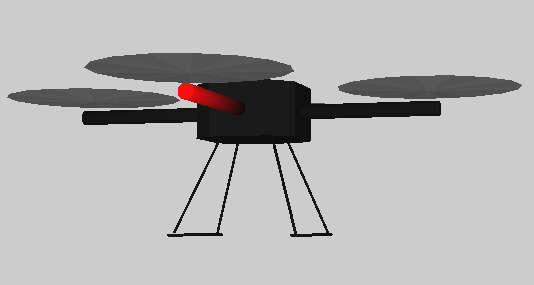
\includegraphics[width=\textwidth]{quadrotor_sim.png}
    \end{subfigure}
    \begin{subfigure}[c]{0.45\textwidth}
      \centering
        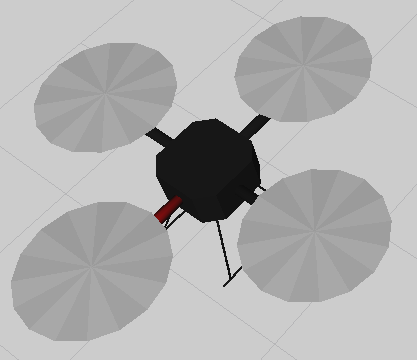
\includegraphics[width=\textwidth]{quadrotor_sim2.png}
    \end{subfigure}
    \caption{Quad-rotor simulated by Hector Quadra
    otor using ROS and gazebo.}
\end{figure}

The dynamics of the quad-rotor are taken from Samir Bouabdallah's work \cite{QuadrotorDynamics}. It includes the flight dynamics, motor dynamics, and thrust calculations required for the system. 

A set of basic controllers are used in our system. These controllers are abstractions of the dynamics model of the system and can be controller using simple inputs such as torque, position or velocity. We used a simple velocity based system for achieving most of the controls.

\section{Reinforcement Learning framework}
Hester T. and Stone P. made a ROS package for their paper on TEXPLORE \cite{Texplore}. The rl-texplore-ros-pkg\footnote{https://github.com/toddhester/rl-texplore-ros-pkg} provides a ROS-topic based isolated service implementing several popular RL-algorithms such as Q-Learning, SARSA etc. As mentioned above, it provided us a loosely coupled environment agent system. However, the package had a few limitations for our system:
\begin{itemize}
	\item The algorithms and the environment implemented was for grid-world like state spaces with a small state space and action space. Our system comprises of continuous states and actions.
	\item  The system didn't integrate gazebo into the environment since the models used didn't require physics simulations.
\end{itemize}

We created our own package \footnote{https://github.com/AbdealiJK/quadrotor\_control}, which depends on hector\_quadrotor and uses Gazebo physics engine. The state space in our system is represented by the position and orientation of the quadrotor, and the action space is a continuous set of actions that can be taken by the quadrotor.

This modified package is able to communicate with gazebo as part of the environment and can use the models of the gazebo simulator and converts it into a state. It also has the ability to run gazebo in finite time steps, pausing the simulator between them.

\subsection*{Agent}
The agent is a ROS node which implements from the abstract class provided in the texplore package \texttt{Agent}. The agent contains a Policy which is updated based on the reward received from the environment. It implements three functions:
\begin{itemize}
	\item \texttt{first\_action}: Represents the action at initiation of the episode.
	\item \texttt{next\_action}: Represents the action at the next time step of the episode.
	\item \texttt{last\_action}: Represents the action at end of the episode. 
\end{itemize} 
The Agent transmits the action using the RLAction message on the topic \texttt{rl\_agent/rl\_action} and this is read by the environment.

\subsection*{Environment}
The environment is a ROS node which implements from the abstract class provided in texplore package \texttt{Environment}. It implements the functions:
\begin{itemize}
	\item \texttt{sensation}: Represents the state or the observation from the environment that the agent gets from the environment. It may comprise of inputs directly from sensors or processed in some way.
	\item \texttt{apply}:  Takes in the action given by an agent through the message and applies it to the environment. 
	\item \texttt{terminal}: The terminal function represents the end of an episode if the environment has reached the desired state. 
	\item  \texttt{reset}: Used to restart the episode. 
\end{itemize} 

The environment transmits the state information using the RLEnv message on the topic \texttt{rl\_env/rl\_state\_reward}. It contains the state information, the scalar reward and information whether the terminal state has been reached.

An environment named Hector Quad-rotor has been implemented which passes the action from the agent to the gazebo environment as a twist state. The sensation function is also implemented in such a way as to wait for gazebo to complete a transition step and return back the observable state from this. For all this a random seed can be set in gazebo to create the repeatable scenarios required by PEGASUS.


\section{Wind implementation}
The wind system needs to be implemented as a continuous system to mimic real environment. The current wind in any direction is given by a zero mean distribution implemented using a uniform distribution. To keep the wind continuous, the random variable sampled from the uniform distribution is added to the current velocity of the wind.
\begin{equation}
\begin{array}{c}
V_{wx} = V_{wx} + K * x_x\\
V_{wy} = V_{wy} + K * x_y\\
V_{wz} = V_{wz} + K * x_z\\	
\end{array}
\end{equation}
where $x_x, x_y and x_z$ represent random variables sampled from a uniform distribution from $[min\_wind\_speed, max\_wind\_speed]$ and K represents a parameter to control the maximum change in wind speed in a time step.

It can be seen that the expectation of $V_{wx}, V_{wy}$ and $V_{wz}$ is average of $min\_wind\_speed$ and $max\_wind\_speed$.

\section{Quadrotor specifications}
The major model parameters used for the simulations are specified here:

\textbf{Mass} = $1.477 kg$

\textbf{Inertia}(in $kgm^2$)

$I_{xx} = 0.01152 \qquad I_{xy} = 0.0 \qquad I_{xz} = 0.0$

$I_{yy} = 0.01152 \qquad I_{yz} = 0.0 \qquad I_{zz} = 0.0218$

\section{Modelling quadrotor payload system}
The quadrotor payload system is modelled using a single link that connects the quadrotor to the payload. The allowed motion relative to the quadrotor for the payload is a hinge like motion. Two joints form part of the system, one joint between the quadrotor and the link to the payload, and the other between the link and the payload. Since Gazebo doesn't have an option to specify ball joints, for a complex joint multiple links would be required.

The payload is set up as a uniform solid cube box of side $0.2m$ and mass $0.2kg$. The connecting link is also a solid box of dimensions $0.02m X 0.02m X 0.3m$ and mass $0.01kg$. All the joints have a certain limit of motion as $\pm 1 radians$.

\section{Pegasus implementation}
Our package also implements Pegasus. Here we briefly have explained the implementation. The \texttt{Pegasus} agent is implemented from the above mentioned Agent class, and implements the methods \texttt{first\_action, next\_action and last\_action}.

The requirement for finding the optimal policy is that we need the gradient of the policy class at the current policy. 

Each of the parameters is changed by a value of $+ and -\epsilon$, and an entire episode is run for multiple times. The reason for running it multiple times is due to the stochasticity in the system. Gradient with respect to each of the parameters is calculated using the 3 point rule, i.e.
\begin{equation}
\nabla_{n_i} \pi(\theta) =  \dfrac {\pi(\theta+\epsilon*n_i)-\pi(\theta-\epsilon*n_i)}  {2 * \epsilon}
\end{equation}

The policy is not updated while finding the gradient for each of the parameters, and is updated after running for $2*N$ episodes where N is the number of parameters. The update rule is given by: 
\begin{equation}
\pi(n_i) = \pi(n_i) + \nabla_{n_i} \pi(\theta) * K \quad \forall n_i \in N
\end{equation}
where K is the policy update parameter, and can be changed to adjust the rate of learning the policy.

\chapter{Position control}

\section{Quadrotor control system}
Position control is implemented by using the abstraction of the quadrotor motion given by the global velocities for motion. The control system is implemented as a on-policy control system, where the system gets better during each iteration and the new policy is used to run the system. The PEGASUS implementation is done for "stable" states ie states where the quadrotor can go and hover/stay. 

\subsection*{State}
The state is comprised of the linear velocities, position and the angular yaw position and velocity of the quadrotor, since these can completely define the stable parts of quadrotor flight. 
The state vector is:
\begin{equation}
  State(S) = [\triangle{x}, \triangle{y}, \triangle{z}, \triangle{\omega}, \dot{x}, \dot{y}, \dot{z}, \dot{\omega}]
\end{equation}
where $\triangle{x}$, $\triangle{y}$, $\triangle{z}$ and $\triangle{\omega}$ represent the relative position of the quadrotor from the current position. The policy used is due to the reason that the control policy should be dependent only on the relative position from the target.  

\subsection*{Action} The action is abstracted out as a set of velocities of the quadrotor in the local frame of the quadrotor. The action used in our implementation are the abstracted velocities after the velocity control. The action vector is:
\begin{equation}
  Action = a = [\dot{x}, \dot{y}, \dot{z}, \dot{\omega}]
\end{equation}

\subsection*{Policy}
The policy class used for the PEGASUS $\pi: S \rightarrow A$ is written as:
\begin{equation}
  Policy = \pi(s) = \left\{
    \begin{array}{c}
      c_1 \times \triangle{x} + c_2 \times \dot{x} \\
      c_3 \times \triangle{y} + c_4 \times \dot{y} \\
      c_5 \times \triangle{z} + c_6 \times \dot{z} \\
      c_7 \times \omega + c_8 \times \dot{\omega} \\
    \end{array}
  \right\}
\end{equation}

\subsection*{Reward}
The reward used is the L1 norm of the deviation from the target. The reward is negative, and so the maximum reward that the quad-rotor can achieve is zero. 
\begin{equation}
  Reward = r(s) = - |x - x_0| - |y - y_0| - |z - z_0| - K \times |\omega - \omega_0|
\end{equation}

\section{Payload control}
Further we explore at controlling the position of a payload. The payload is suspended on the quadrotor with certain degree of motion allowed at the joint, allowing some relative motion between the two.

\begin{figure}[H]
  \centering
    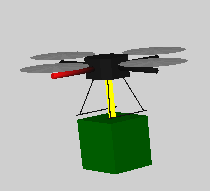
\includegraphics[width=0.4\textwidth]{payload_sim.png}
    \caption{Quadrotor with an additional payload.}
\end{figure}

\section{Learning time optimal policy}
A discounted reward is used to find the return of the policy using Pegasus. A good discount rate ensures that the quadrotor reaches its target as soon as possible, and at the same time with no oscillations.

%%%%%%%%%%%%%%%%%%%%%%%%%%%%%%%%%%%%%%%%%%%%%%%%%%
\chapter{Trajectory control}
We use the basic controller that we set up to control the quadrotor's trajectory. A trajectory is set up as a set of stable states that the quadrotor has to go through. A simple representation of a trajectory is represented in this image where the marked points may be critical "checkpoints" or just guiding points for the motion needed.


\section{Checkpoints based trajectory control}
The quadrotor needs to go through a set of ordered checkpoints that define the trajectory. The checkpoints are considered as crossed if the quadrotor has moved "close enough" to the checkpoint. As soon as the quadrotor reaches a checkpoint, its target is set to the following checkpoint. This sort of method is essential in a case where checkpoints and closeness to them have a real world meaning, for example the system needs to be in a certain range to allow the payload to be removed.

\begin{figure}[H]
  \centering
    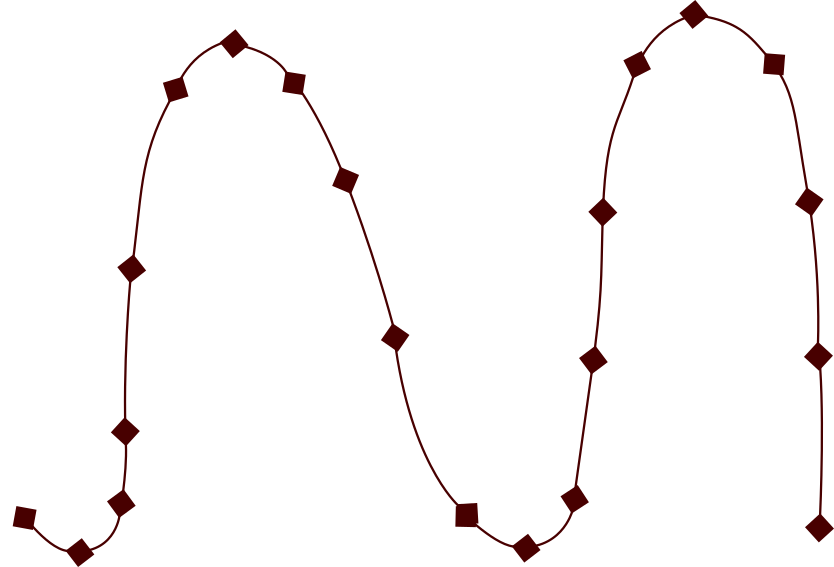
\includegraphics[width=0.35\textwidth]{trajectory.png}
    \caption{Sample checkpoint based trajectory. This trajectory was generated using a simple drawing tool. Trajectories can be generated with mathematical representations as in our packages, or using CAD software.}
\end{figure}

\subsection*{Representation}
The format representation of a quadrotor having crossed the checkpoint if its position is within a spatial neighbourhood of the checkpoint can be written as:
\begin{equation} \begin{split}
  |x - x_c| &< \epsilon_x \\
  |y - y_c| &< \epsilon_y \\
  |z - z_c| &< \epsilon_z \\
  |\omega - \omega_c| &< \epsilon_\omega
\end{split} \end{equation}
where $\epsilon_x$, $\epsilon_y$, $\epsilon_z$ and $\epsilon_\omega$ are the real world ranges that need to be considered and the vector
\begin{equation}
  [x_c, y_c, z_y, \omega_c]
\end{equation}
represents the checkpoint comprising the desired position and orientation of the quadrotor.

\begin{figure}[H]
  \centering
    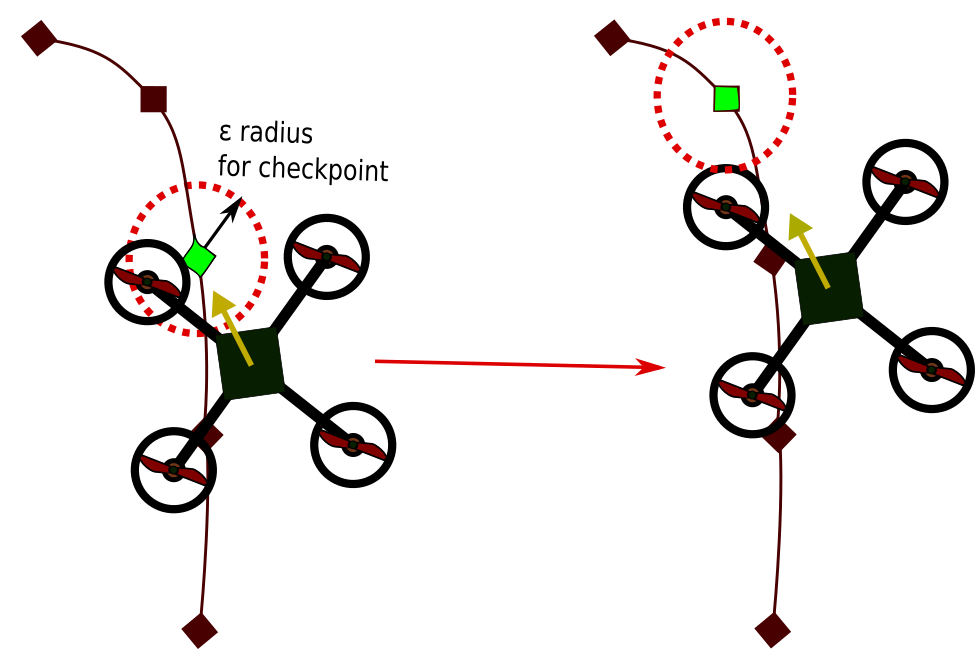
\includegraphics[width=0.9\textwidth]{Checkpoint_trajectory.png}
     \caption{Shows checkpoints for a certain trajectory. The targetis set as the next checkpoint once the quadrotor passes an $\epsilon$ neighbourhood of the current checkpoint.}
\end{figure}

	
\subsection*{Issues}
The checkpoint method ensures that the quadrotor has to follow certain checkpoints in order, and if the quadrotor misses a checkpoint by greater than the $\epsilon$ distance and the projection of the current position on the trajectory is closer to the next checkpoint, the quadrotor still tries to go to the older checkpoint.

\begin{figure}[H]
  \centering
    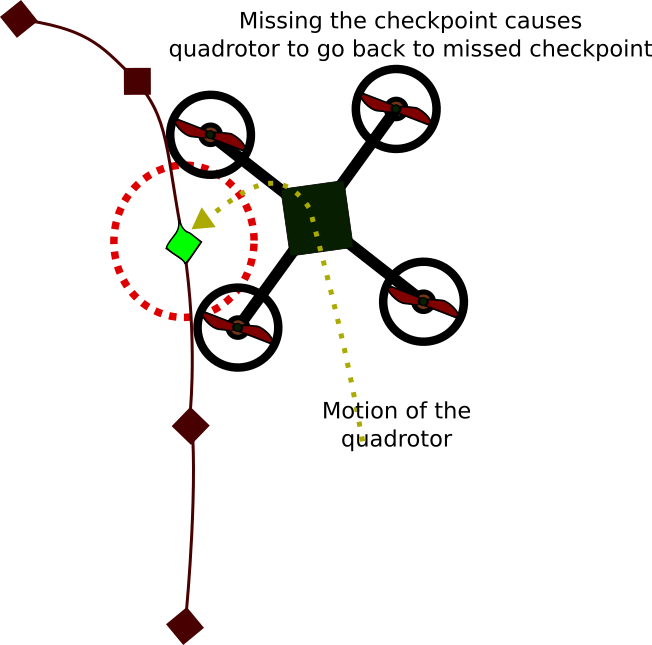
\includegraphics[width=0.5\textwidth]{Checkpoint_trajectory_miss.png}
     \caption{Schematic shows that on missing the region of the current checkpoint, the quadrotor tries to again reach the point which isn't suitable for being on the trajectory.}
\end{figure}


Another drawback of this system is that the overall path isn't time optimal, the quadrotor's aim is to reach the next checkpoint in the best possible way. The motion is expected to have acceleration while far from checkpoint and deceleration when near the next checkpoint.

%%%%%%%%%%%%%%%%

\section{Pursuit based trajectory control}

The aim here is to consider the complete trajectory function with time. The target is changed at every step with the expected position of the quadrotor. The target is actually defined by where the quadrotor is expected to move to.

Although the control is much more smoother with respect to the checkpoints method, it is a complex task to design the pursuit trajectory in a real world system. Incorrectly estimating the lead time of the trajectory can lead to the system being much off the trajectory. Additionally, there is no driving force in this method to reinstate the system back to the desired trajectory.

%%%%%%%%%%%%%%%%
\section{Waypoints based method}
Waypoint method also uses a set of points for defining the trajectory, and as the name suggests, it doesn't rely on the quadrotor moving through those points. It gives guiding points for controlling the motion of the system without restricting the motion in case there is a deviation in the motion. 

\begin{figure}[H]
  \centering
    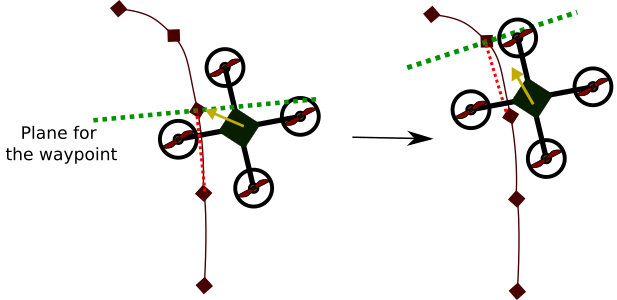
\includegraphics[width=0.9\textwidth]{Waypoints_trajectory.png}
    \caption{Using the waypoint technique for control, the quadrotor isn't close to the actual position of the waypoint but passing the plane through the waypoint allows the waypoint to be shifted to the next one}
\end{figure}

\subsection*{Implementation}
The quadrotor has gone through a waypoint, if it has passed through the plane of the waypoint normal to the line joining the previous and current waypoint. Here, although the quadrotor policy still tries to make it move towards the next point in the trajectory, being off the trajectory doesn't affect it's future motion and it keeps going towards the next point. 

At the same time, this error isn't additive and hence the deviations in trajectory during reaching a waypoint can be ignored. This gives overall a smoother position control over the trajectory it is trying to follow.

The waypoint method still faces the issues faced by checkpoint method of unstable motion, i.e. the quadrotor would accelerate and decelerate each time depending on how far it is from the waypoint.

To some extent, this can be solved by using a plane at a distance of $\epsilon$ from the waypoint plane and parallel to it, where the waypoint gets shifted to the next one. This will ensure that though the quadrotor is trying to reach the waypoint plane, it stops trying to reach it as soon as it reaches the dummy plane, and then tries to reach the next waypoint plane.
\begin{figure}[H]
  \centering
    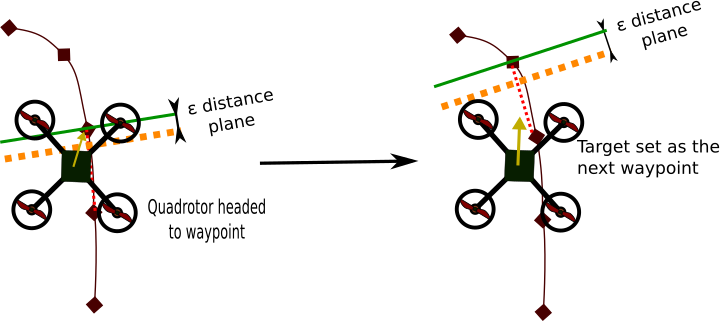
\includegraphics[width=\textwidth]{Waypoints_epsilon.png}
    \caption{Using an $\epsilon$ shifted plane parallel to the waypoint plane, helps maintain a smoother motion for the system.}
\end{figure}

\subsection*{Results}
\begin{figure}[H]
  \centering
    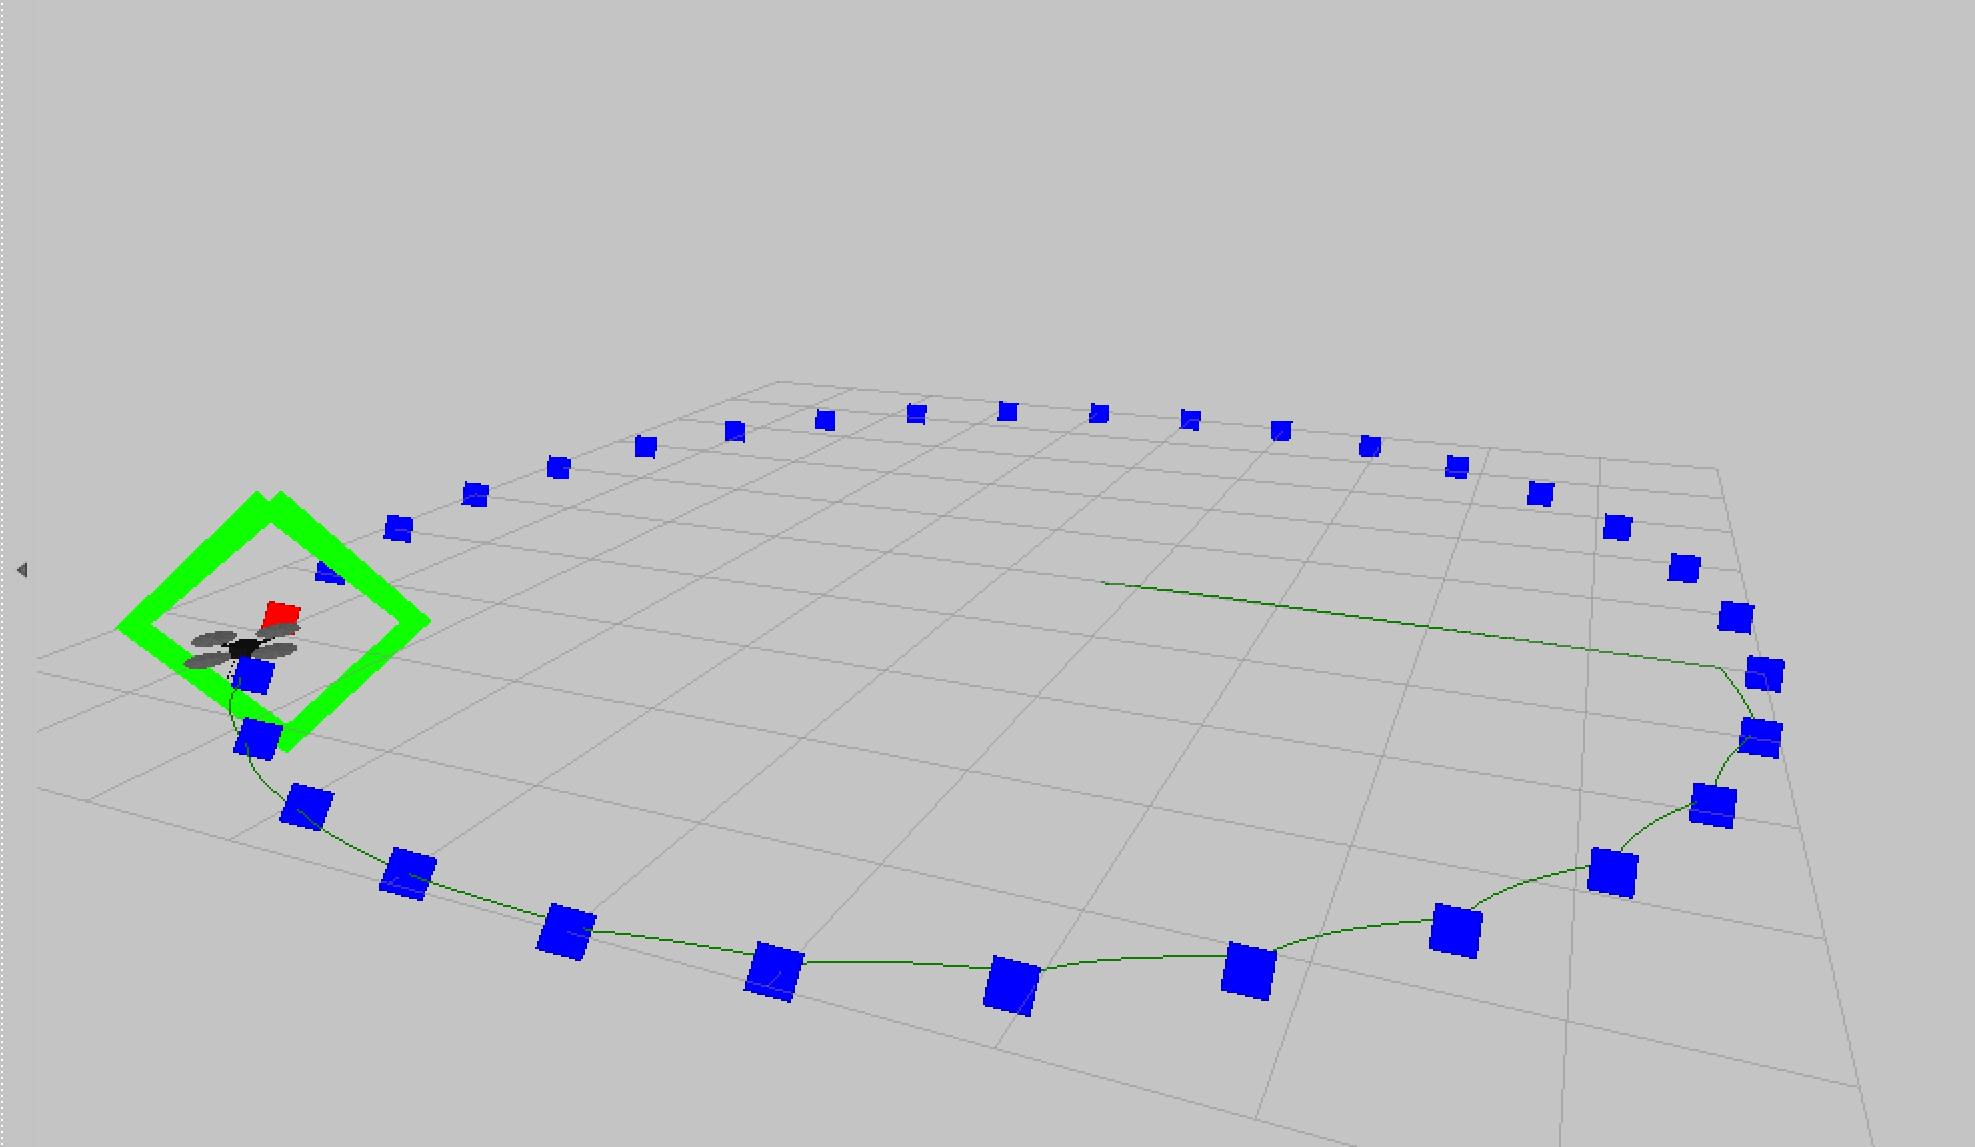
\includegraphics[width=\textwidth]{Waypoints_plane.png}
    \caption{Plane based representation for waypoints method. Red marker represents the waypoint the quadrotor is trying to reach, and the green square represents the plane that needs to be crossed to switch to the next waypoint. The blue markers represent the entire trajectory that needs to be followed}
\end{figure}

Impact of using an $\epsilon$ shifted plane as the waypoint plane can be seen from the figure below. A longer $\epsilon$ distance would lead to a much more stable trajectory with lesser variations in speed. The first figure shows Waypoints method($\epsilon=0$), the trajectory achieved is much better in terms of the motion with respect to the trajectory, but the epsilon shifted method results in a much more "loose" trajectory achieved i.e. the total error with respect to the target trajectory is higher. 

\begin{figure}[H]
  \centering
  \begin{subfigure}[t]{0.45\textwidth}
    \centering
      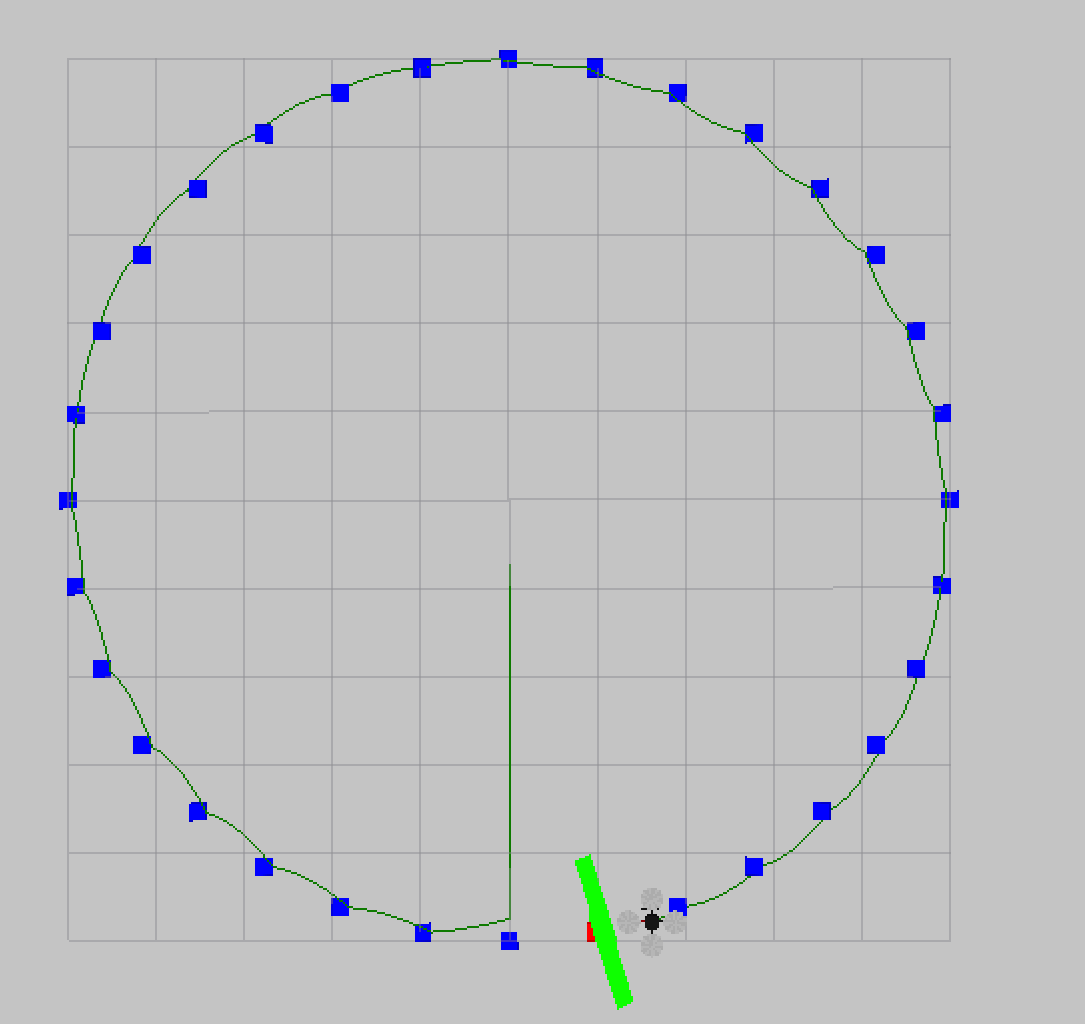
\includegraphics[width=\textwidth]{Waypoints.png}
      \caption{Waypoints method}
  \end{subfigure}
  \begin{subfigure}[t]{0.45\textwidth}
    \centering
      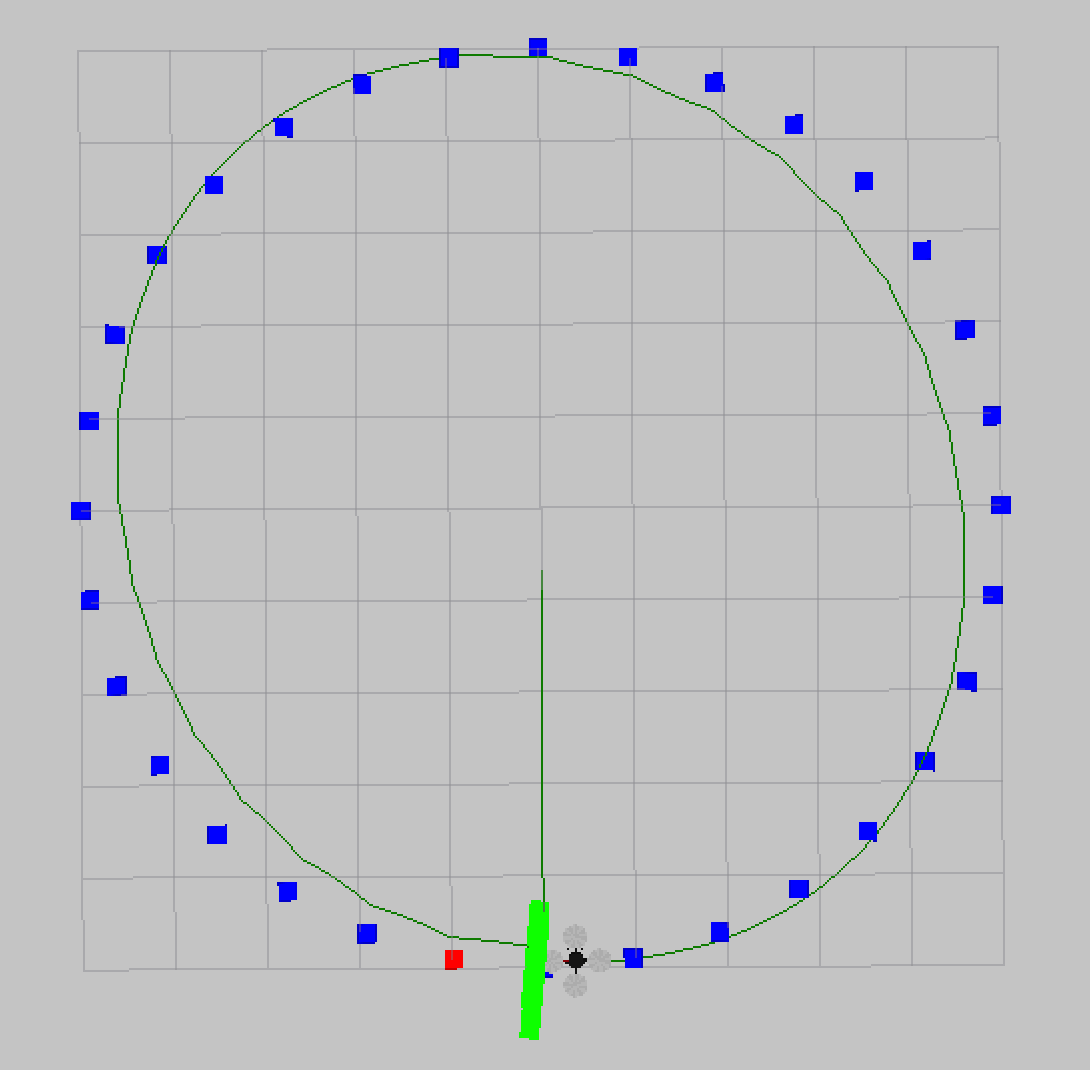
\includegraphics[width=\textwidth]{Waypoints_0_9.png}
      \caption{Waypoints with a shifted $\epsilon$ plane}
  \end{subfigure}
  \caption{Quadrotor simulation moving in a circular trajectory with the waypoint technique.}
\end{figure}

\subsection*{Smoothness of motion}
Using the $\epsilon$ plane solves the problem of rapid change in speeds of the quadrotor and achieves an overall smoother motion. Both checkpoints based method and the waypoints method have very unstable and jerky motions.
\begin{figure}[H]
  \centering
  \begin{subfigure}[t]{0.48\textwidth}
    \centering
      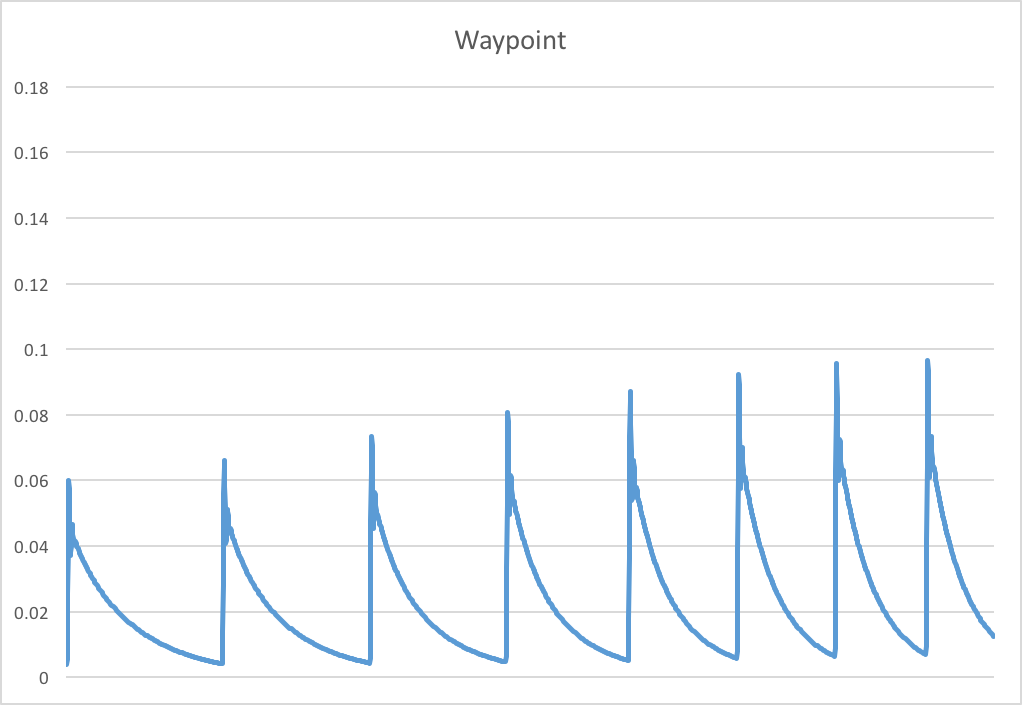
\includegraphics[width=\textwidth]{Waypoints_speed.png}
      \caption{Speed(in m/s) for waypoints based trajectory}
  \end{subfigure}
  \quad
  \begin{subfigure}[t]{0.48\textwidth}
    \centering
      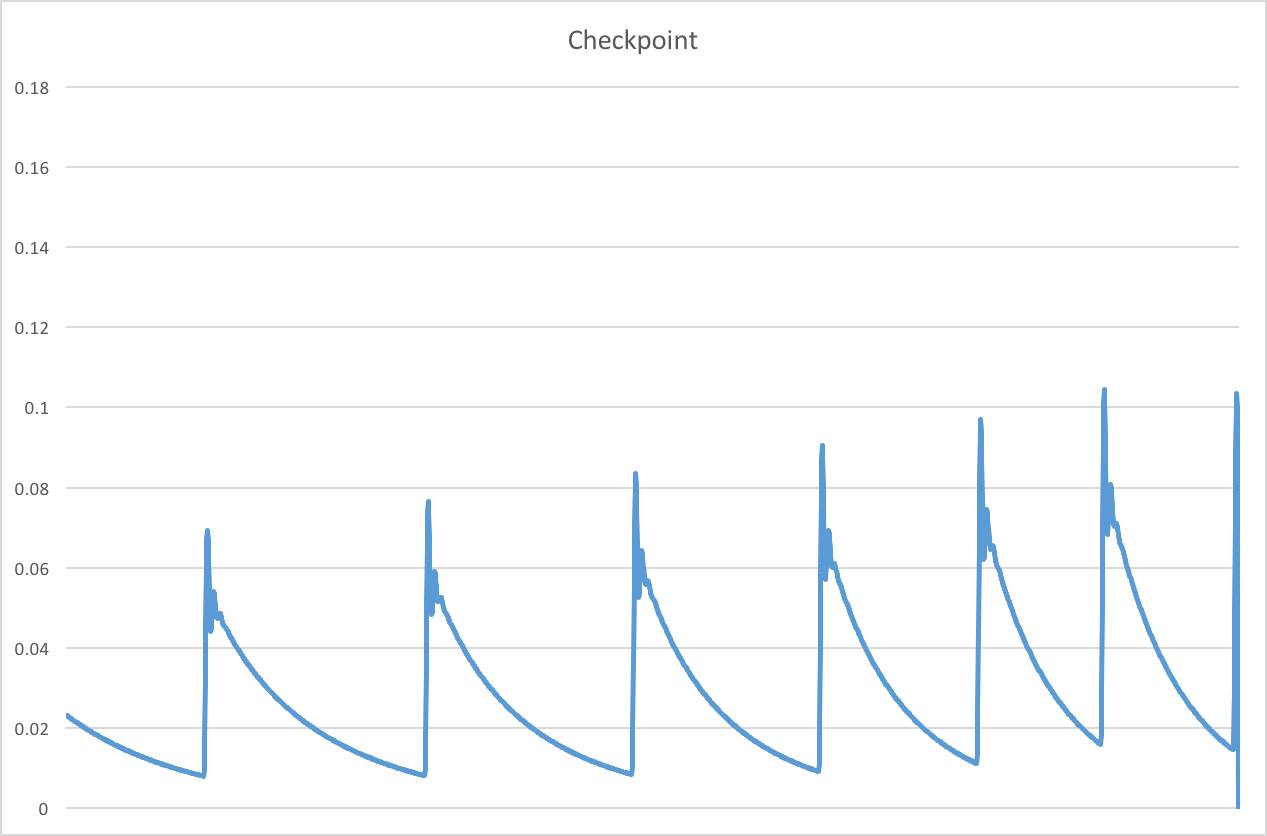
\includegraphics[width=\textwidth]{Checkpoint_speed.png}
      \caption{Speed(in m/s) for checkpoints based trajectory}
  \end{subfigure}
  \caption{Variation of speed for waypoint and checkpoint trajectories.}
\end{figure}
As seen from the figure above, both checkpoints and waypoints based method face the problem of variation of speed while following a trajectory. The speed falls to zero at times and again increases during the course of motion of the quadrotor. The near-zero speeds are reached as the quadrotor is near the checkpoint or the waypoint plane.
\begin{figure}[H]
  \centering
    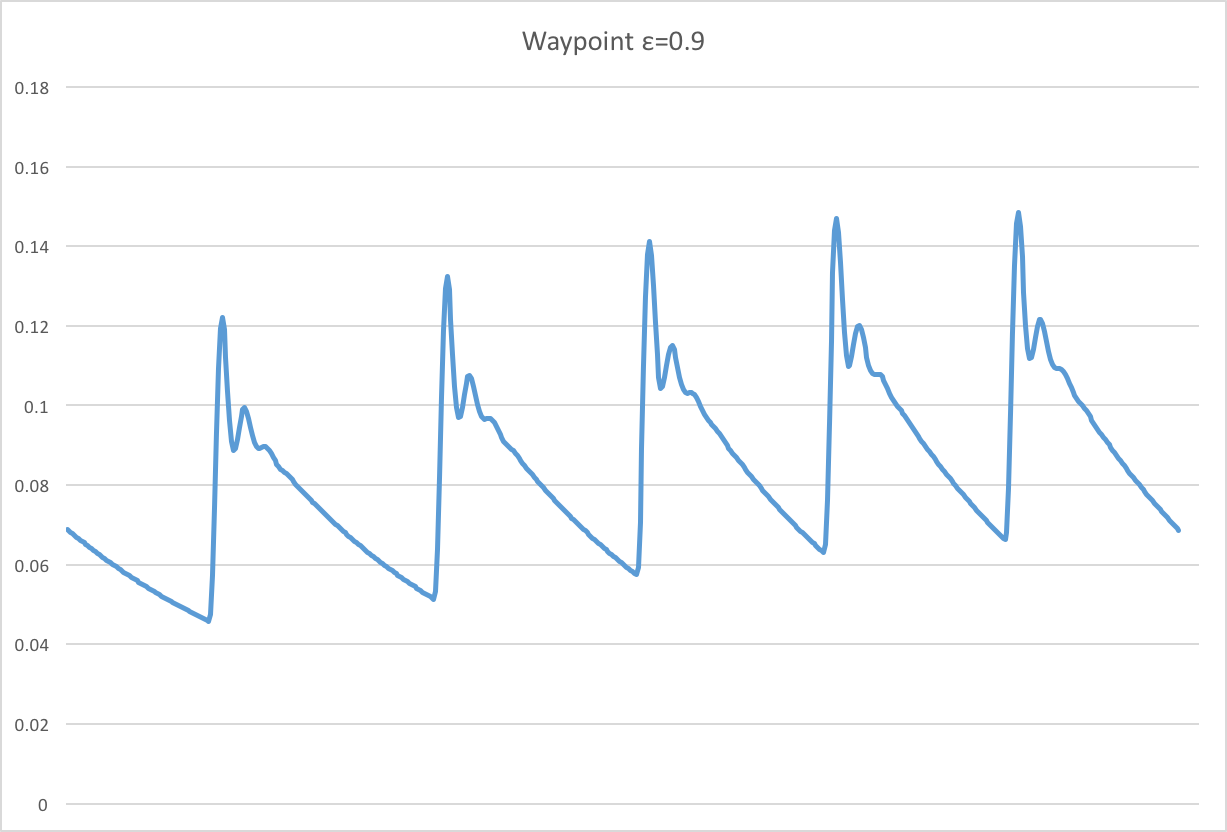
\includegraphics[width=0.8\textwidth]{Waypoints_speed_0_9.png}
    \caption{Speed(in m/s) for waypoints based trajectory with an epsilon plane.}
\end{figure}
As seen from the figure above, there are some variations in the speed of the quadrotor during the motion, however, the speed never falls to zero, and the motion is much more stable. This can be made further stable by taking a maximum speed for the quadrotor as the lower limit of speed in the graph. That would give a perfectly smooth motion for the quadrotor.

\subsection*{Effect of wind}
Wind used in our system causes certain effects on both the waypoints and the epsilon plane based waypoints based methods. The general behaviour remains the same, the waypoints method is better at achieving the trajectory in the presence of wind and epsilon plane based method is able to achieve a much more stable trajectory for the quadrotor.
\begin{figure}[H]
  \centering
  \begin{subfigure}[t]{0.45\textwidth}
    \centering
      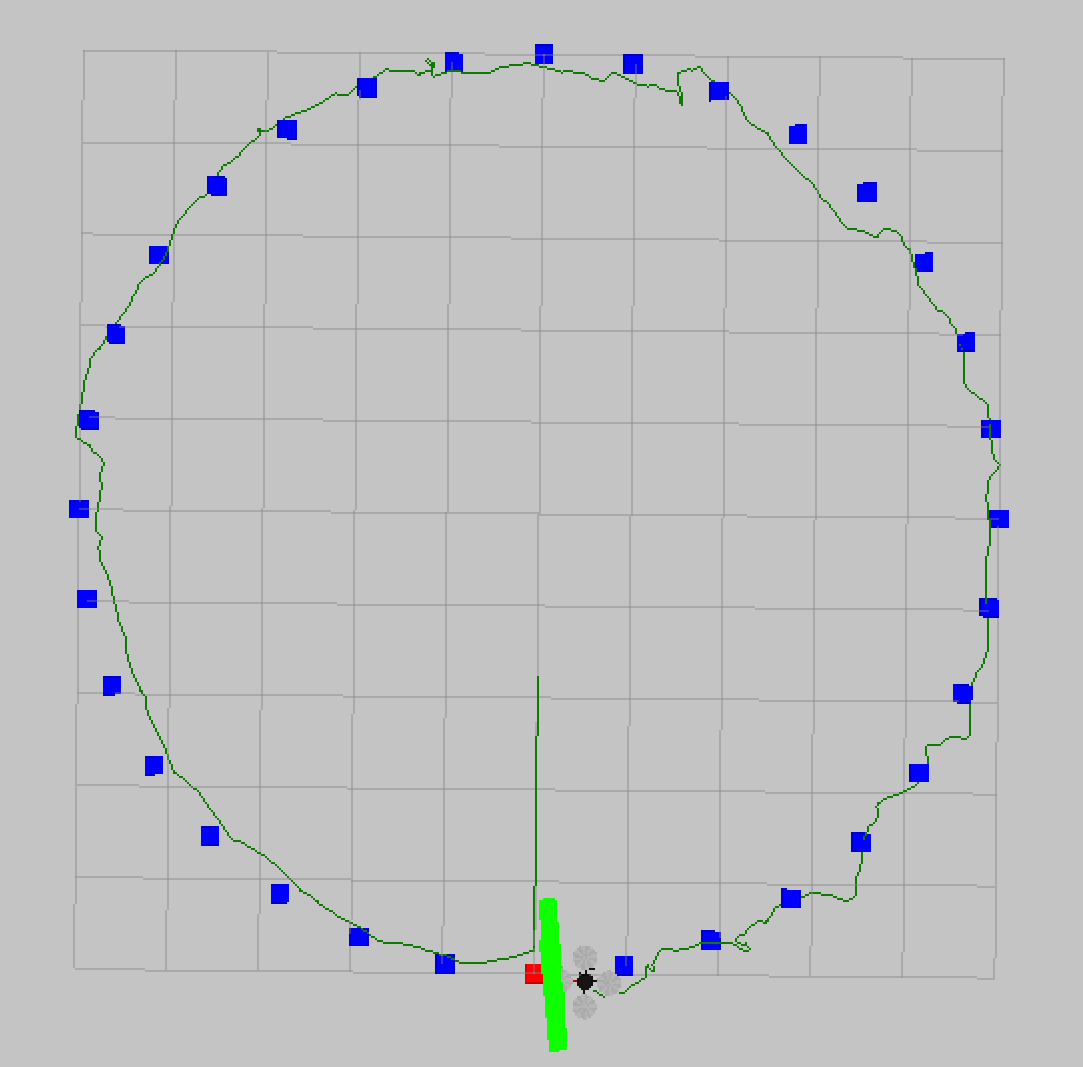
\includegraphics[width=\textwidth]{Waypoints_wind.png}
      \caption{Waypoints method}
  \end{subfigure}
  \begin{subfigure}[t]{0.49\textwidth}
    \centering
      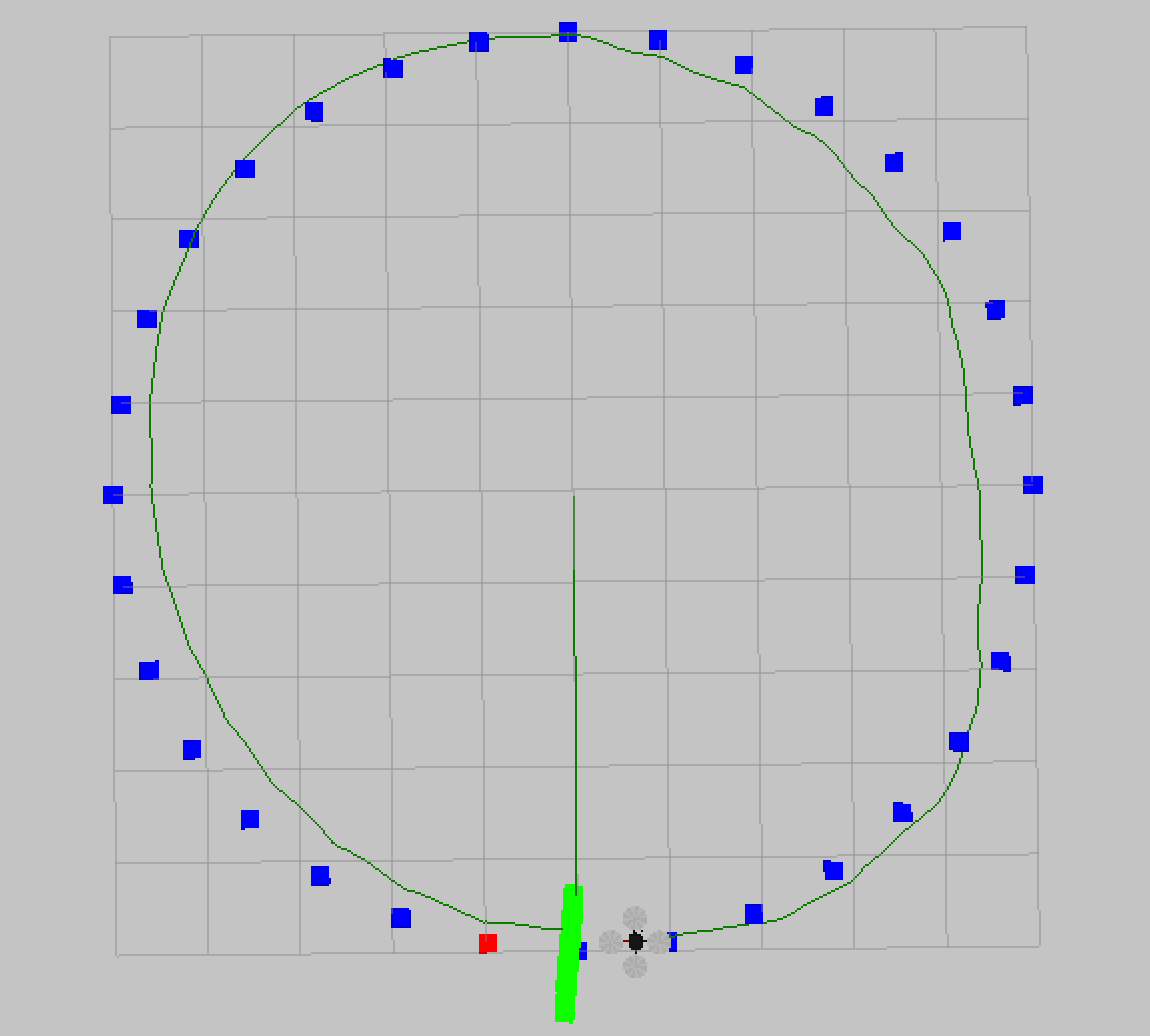
\includegraphics[width=\textwidth]{Waypoints_0_9_wind.png}
      \caption{Waypoints with a shifted $\epsilon$ plane}
  \end{subfigure}
  \caption{Effect of wind on Quadrotor simulation moving in a circular trajectory with the waypoint technique.}
\end{figure}


%%%%%%%%%%%%%%%%
\section{ Pure Pursuit}
Pure Pursuit algorithm comes from control theory domain, where the setpoint is always a point on the trajectory at a lookahead distance. The lookahead distance represents how far along the path should the system consider while moving ahead. The motion velocity and direction are dependent on the path and the lookahead distance. The setpoint in this system is always moving as the system moves.

In case of Pure Pursuit, the current position of the system is projected on the trajectory that it needs to follow, and the setpoint is set at lookahead distance on the trajectory. The direction of motion of the system is towards the setpoint. 

\begin{figure}[H]
  \centering
    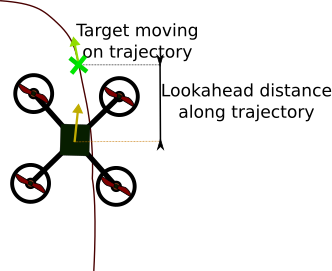
\includegraphics[width=0.5\textwidth]{Pure_Pursuit.png}
    \caption{Pure Pursuit technique representation. The target is dynamically generated and moves on the trajectory depending on the position of the quadrotor.}
\end{figure}

\subsection*{Advantages and limitations}
This system solves some of the problems of the above mentioned path tracking algorithms.
\begin{itemize}
	\item The motion during the pursuit trajectory is much more stable, since the setpoint always moves with the motion of the system. There is no acceleration or deceleration observed during the course of the motion.
	\item Able to control how fast/slow the system should move using the lookahead distance parameter. 
	\item The motion is time-optimal, since the original motion for reaching the setpoint is time-optimal. The speed of the motion can be easily controlled by the lookahead distance parameter.
	\item The controller always tries to get the system back on the desired trajectory, though the motion may be oscillatory in some cases. 
\end{itemize}


However, it introduces some issues in the system, the parameter Lookahead distance needs to be optimized for the trajectory selected, and to follow the trajectory, might need to be different for different segments. Setting the Lookahead parameter incorrectly might cause the motion to be highly deviated, even with an optimal control system for reaching a checkpoint. 
For example, a curve with a big radius of curvature can be covered with a higher lookahead though a sharp turn needs a very small lookahead distance in order to follow the path.

\begin{figure}[H]
  \centering
  \begin{subfigure}[t]{0.3\textwidth}
    \centering
      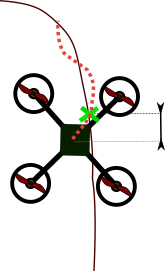
\includegraphics[width=\textwidth]{Pure_Pursuit_short.png}
      \caption{Short lookahead distance}
  \end{subfigure}
\qquad
  \begin{subfigure}[t]{0.3\textwidth}
    \centering
      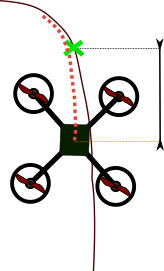
\includegraphics[width=\textwidth]{Pure_Pursuit_long.png}
      \caption{Large lookahead distance}
  \end{subfigure}
  \caption{Comparison of motion using Pure Pursuit algorithm with different lookahead distances.}
\end{figure}

As represented by the schematic, a shorter lookahead distance leads to being closer to the path, but the motion can be jerky, and a longer lookahead leads to a stable and smooth path, but the time taken to reach the path is more. Additionally, the lookahead distance also defines the speed of the quadrotor, so a shorter lookahead is going to be a slower motion with a lot more of acceleration-deceleration.


\subsection*{Implementation}
Implementation of Pure Pursuit in case of a quadrotor doesn't need the complexity of finding the arc to move the quadrotor in, due to the fact that the quadrotor can move in the XY plane without any change in orientation of the system. Hence the control becomes extremely simple.

The implementation for the Pure Pursuit system is done by projecting the current position of the quadrotor on the desired trajectory. This is done in order to easily find out the target point without mathematical complexity of solving for the lookahead point. The target point is chosen as point on the trajectory at lookahead distance from the current position of the projection point. Finally the quadrotor's velocity is set using our PEGASUS based controller.
\begin{figure}[H]
  \centering
    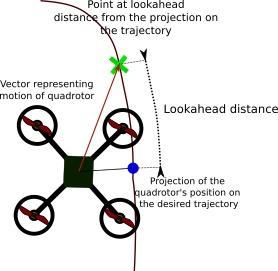
\includegraphics[width=0.5\textwidth]{Pure_Pursuit_implementation.png}
    \caption{Implementation of Pure Pursuit algorithm}
\end{figure}

\subsection*{Results}
Using different lookahead distances, we can vary both the speed of motion of the quadrotor and the "correctness" of the system on the trajectory.
\begin{figure}[H]
  \centering
    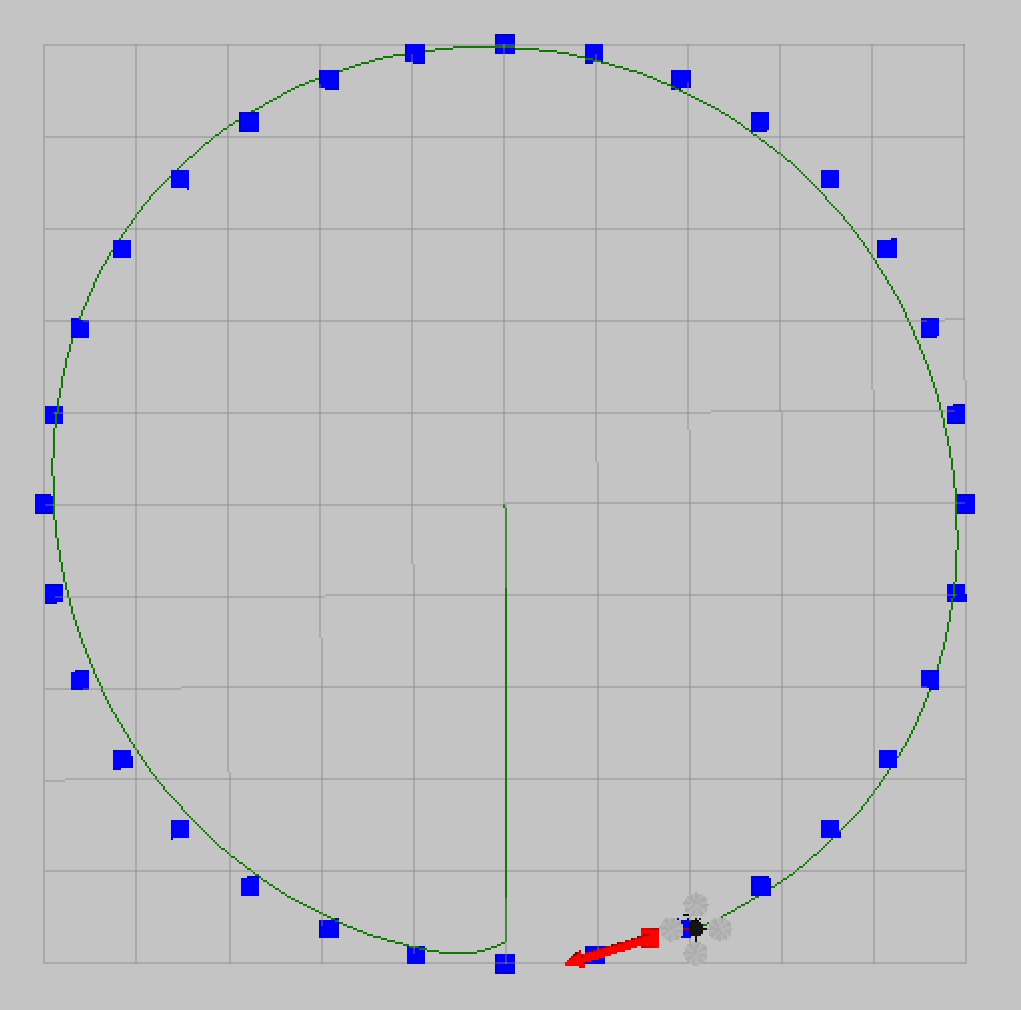
\includegraphics[width=0.7\textwidth]{Pure_Pursuit_0_5.png}
    \caption{Pure Pursuit with lookahead=0.5}
\end{figure}
A short lookahead distance leads to the motion followed being much closer to the original trajectory, and the motion is slower.

\begin{figure}[H]
  \centering
    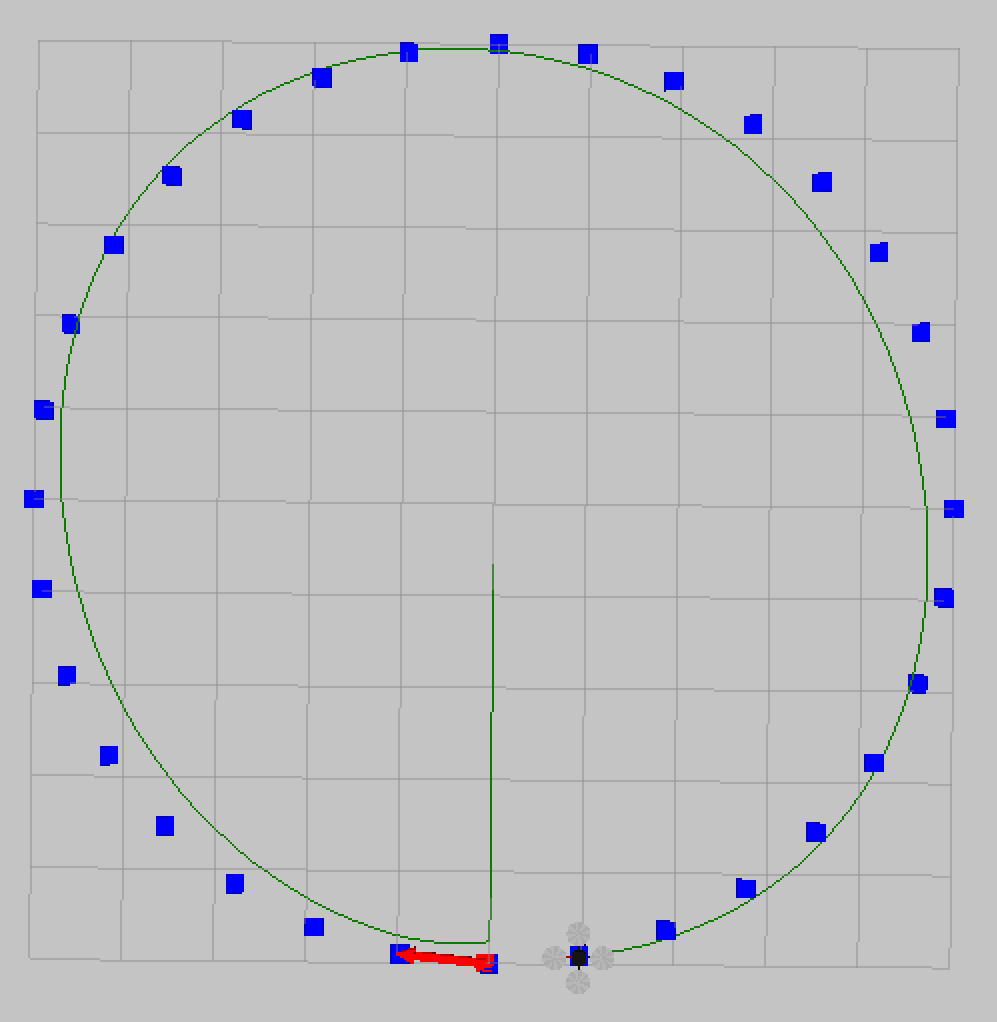
\includegraphics[width=0.7\textwidth]{Pure_Pursuit_1.png}
    \caption{Pure Pursuit with lookahead=1}
\end{figure}
On the other hand, a long lookahead distance used would compromise on the motion of the quadrotor but at the same time would help to achieve the motion much faster.

\subsection*{Stable motion using Pure Pursuit}
\begin{figure}[H]
  \centering
  \begin{subfigure}[t]{0.48\textwidth}
  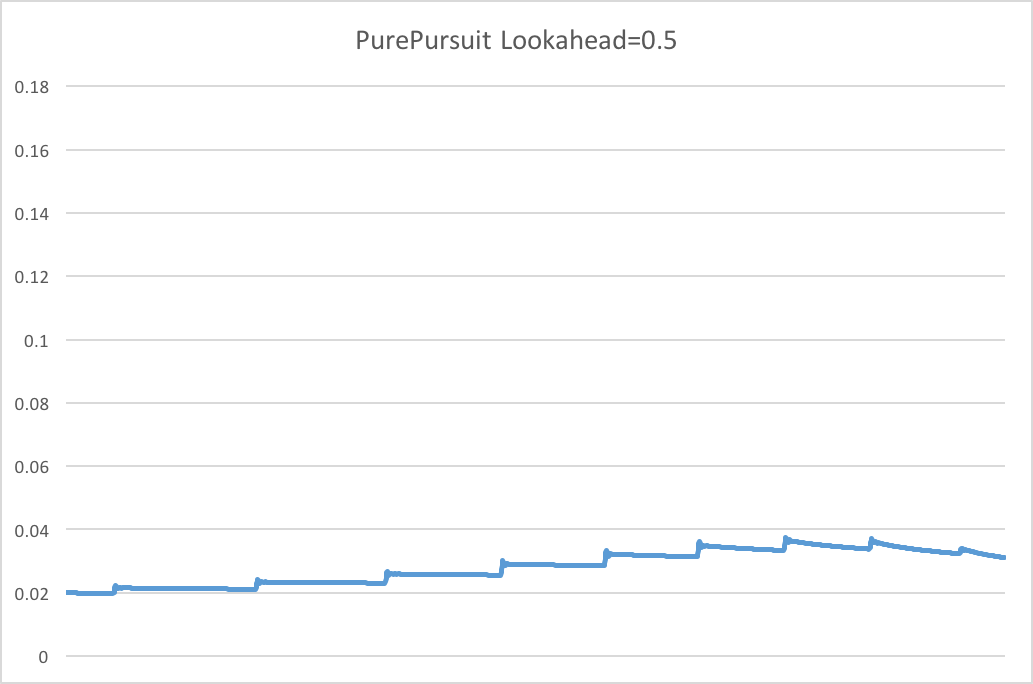
\includegraphics[width=\textwidth]{Pure_Pursuit_speed_0_5.png}
      \caption{Short lookahead distance = 0.5}
  \end{subfigure}
  \begin{subfigure}[t]{0.48\textwidth}
    \centering
      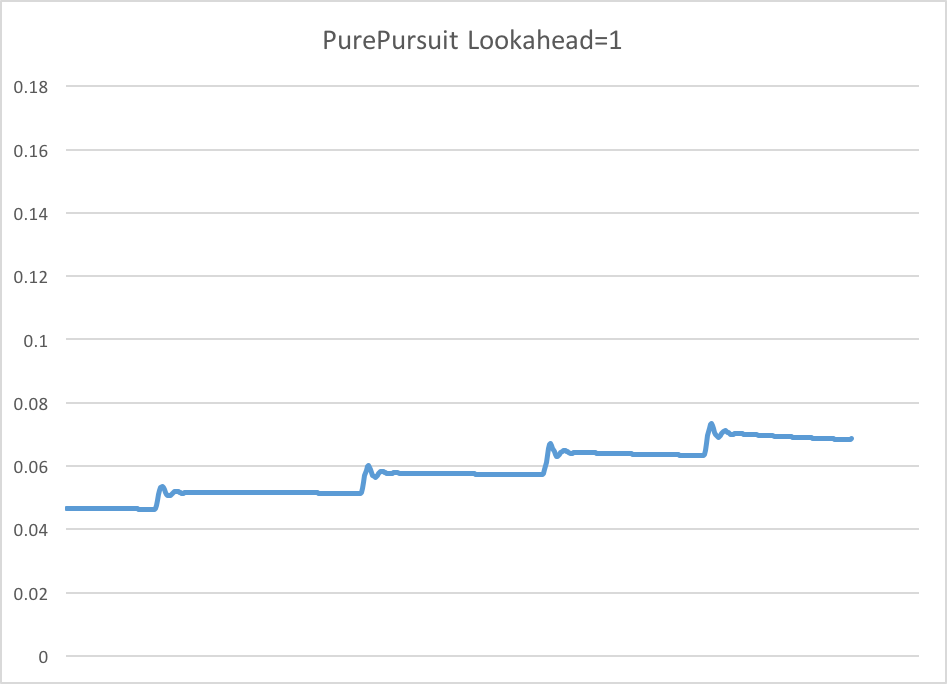
\includegraphics[width=\textwidth]{Pure_Pursuit_speed_1.png}
      \caption{Large lookahead distance = 1}
  \end{subfigure}
  \caption{Speed(in m/s) of motion of quadrotor following Pure Pursuit trajectory tracking. Scale is same as for Waypoints/Checkpoints case.}
\end{figure}
It can be seen that the motion in this case is much more stable as compared to waypoint and checkpoint methods due to the fact that the target changes dynamically and based on the current position. The speed of the quadrotor is governed by the lookahead distance. Using a shorter lookahead distance, slower speeds are achieved, while using a longer lookahead, the speed is faster.

\begin{figure}[H]
  \centering
  \begin{subfigure}[t]{0.45\textwidth}
  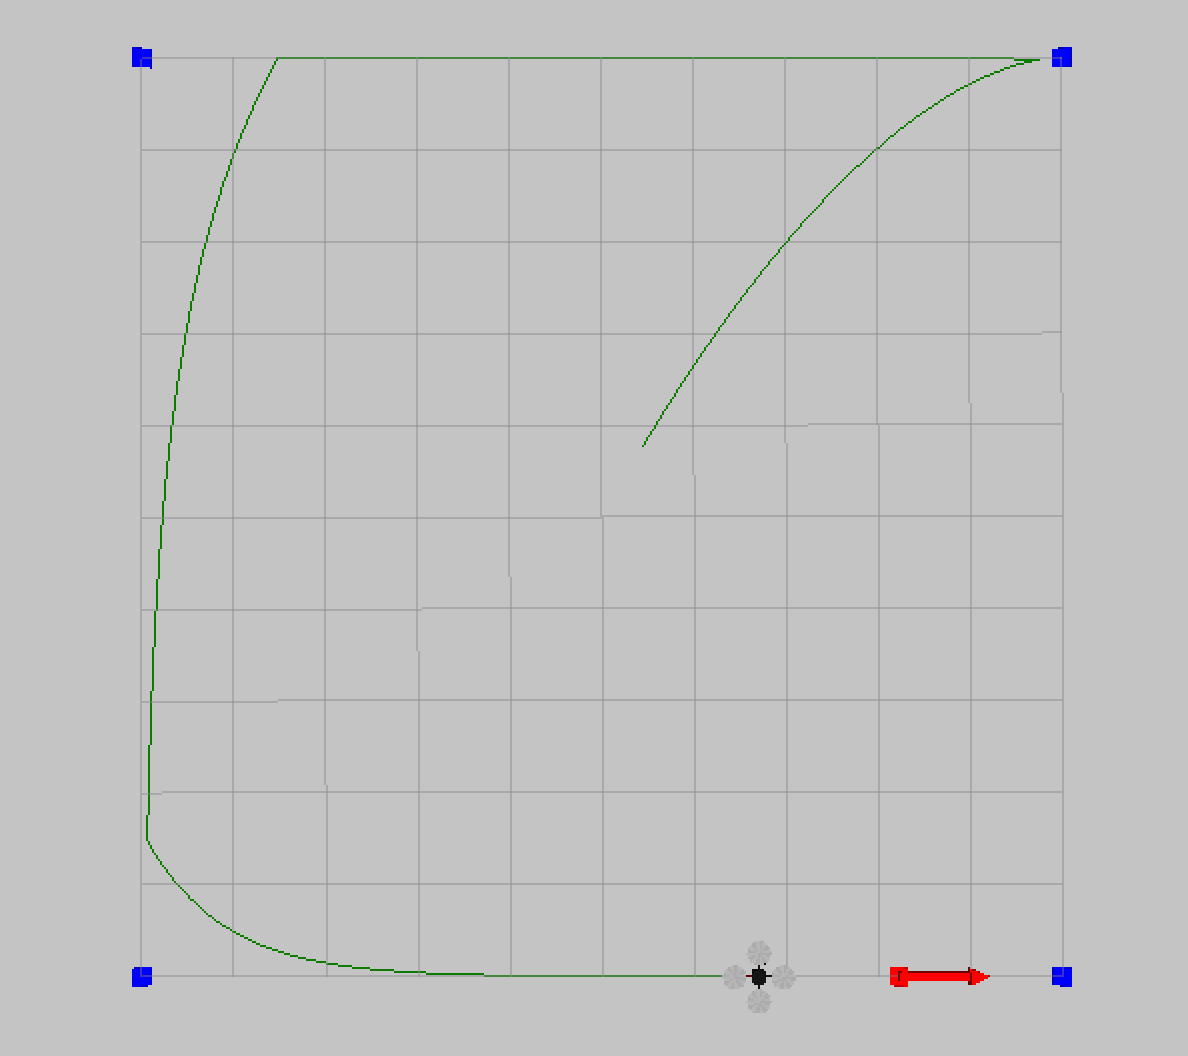
\includegraphics[width=\textwidth]{Pure_Pursuit_rect.png}
      \caption{Rectangle trajectory with minimum number of points, notice the effect of a long lookahead at the corners.}
  \end{subfigure}
  \begin{subfigure}[t]{0.45\textwidth}
    \centering
      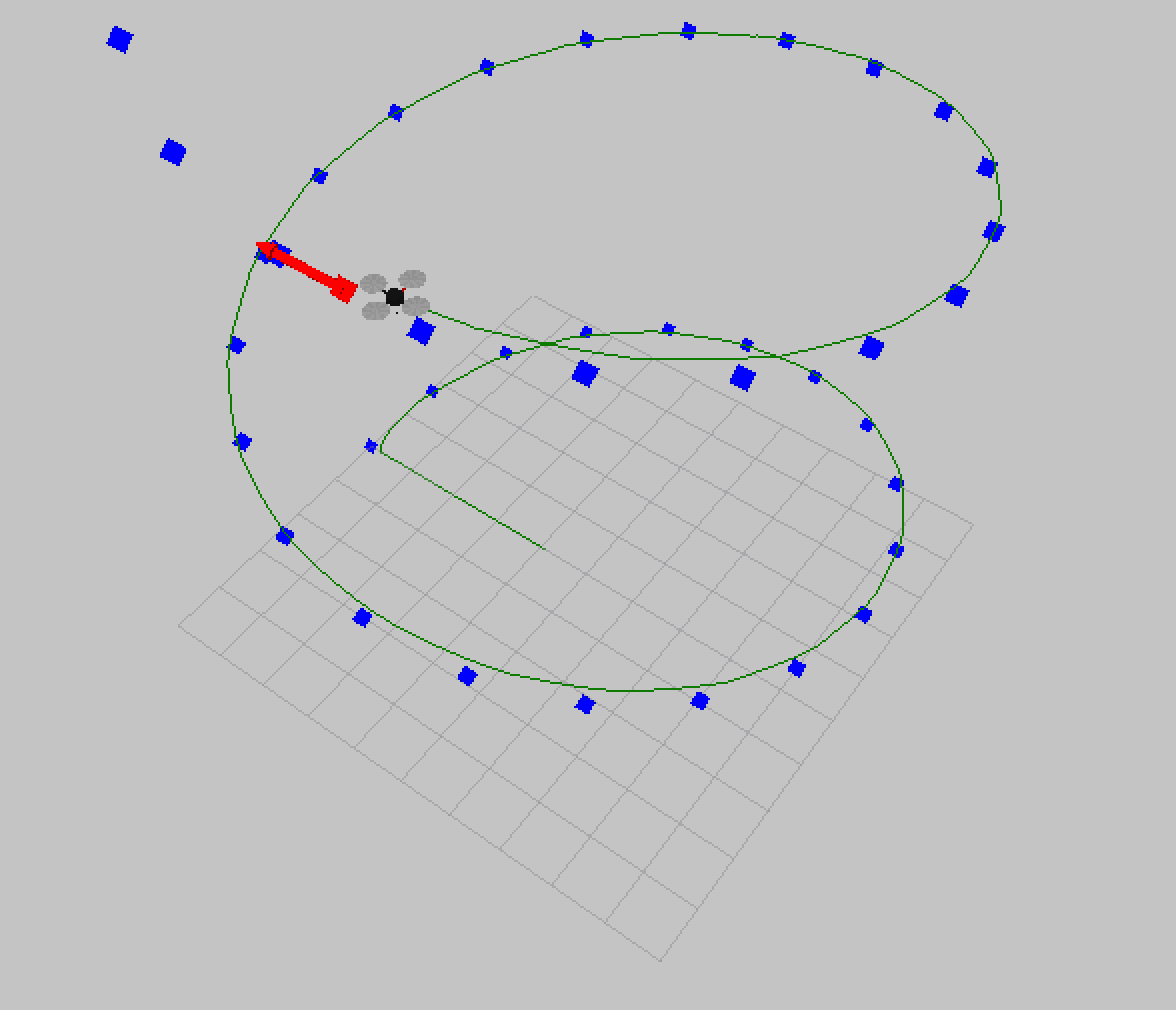
\includegraphics[width=\textwidth]{Pure_Pursuit_helix.png}
      \caption{Helical trajectory}
  \end{subfigure}
  \caption{Different trajectories using Pure Pursuit.}
\end{figure}


\subsection*{Payload control}
As mentioned in the chapter on Position control, the focus is here on controlling the Position and orientation of the Payload and not the Quadrotor. 

\begin{figure}[H]
  \centering
    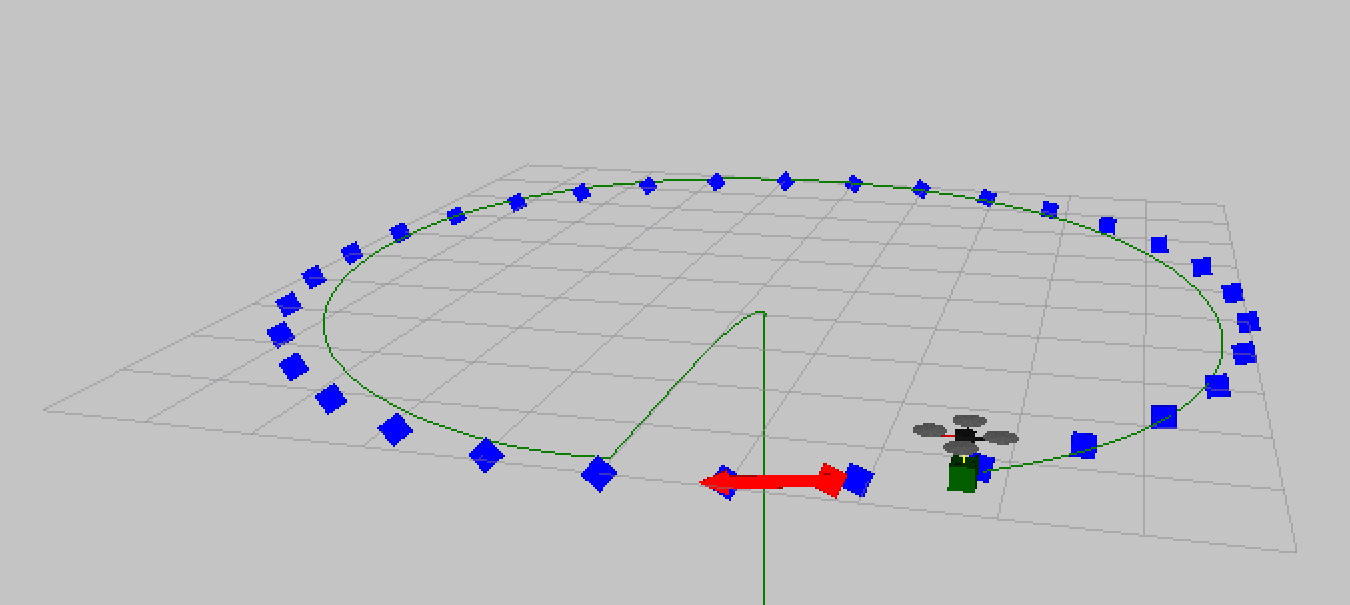
\includegraphics[width=0.7\textwidth]{Pure_Pursuit_payload.png}
    \caption{Trajectory control for payload}
\end{figure}

The PurePursuit algorithm proved to be much better than any other algorithms in the case of Payload and trajectories, and we report the results of only the PurePursuit case. 
\begin{figure}[H]
  \centering
  \begin{subfigure}[t]{0.48\textwidth}
  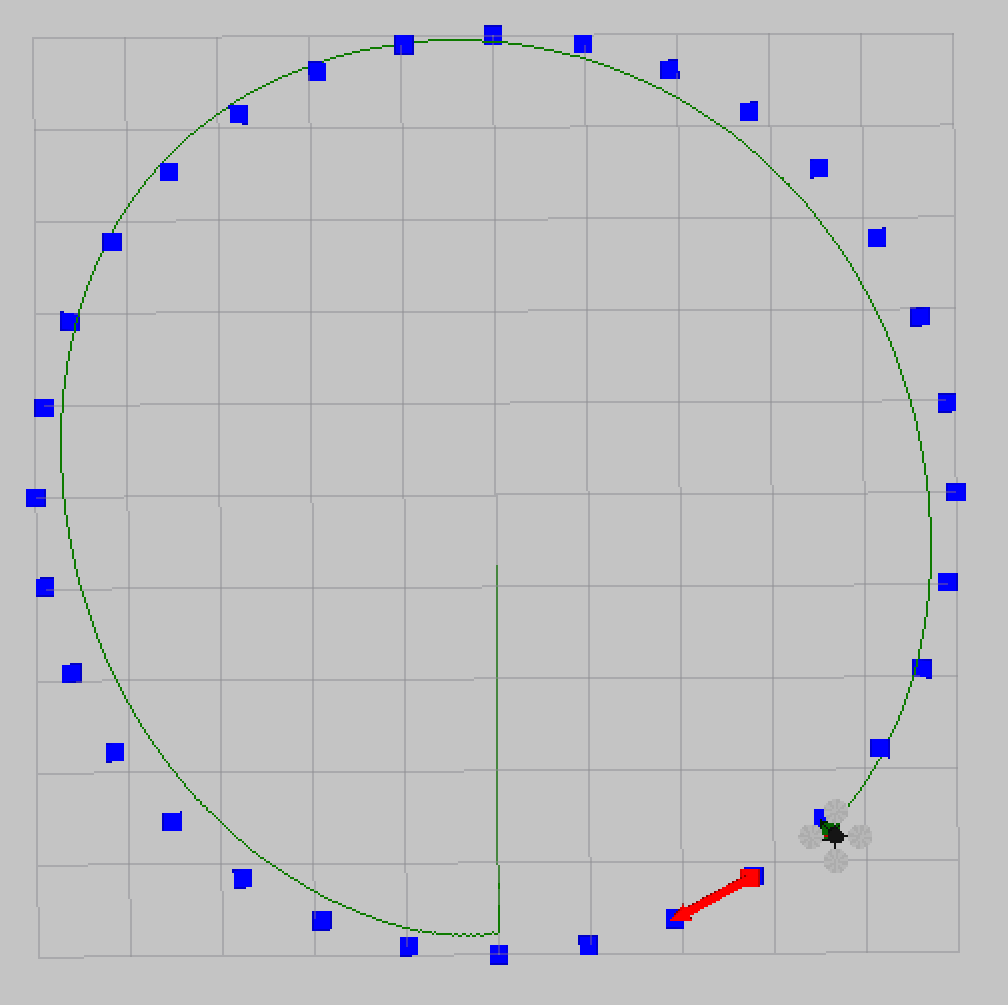
\includegraphics[width=\textwidth]{Pure_Pursuit_1_payload_0_1.png}
      \caption{Payload mass=0.1kg, Lookahead=1m}
  \end{subfigure}
  \begin{subfigure}[t]{0.48\textwidth}
    \centering
      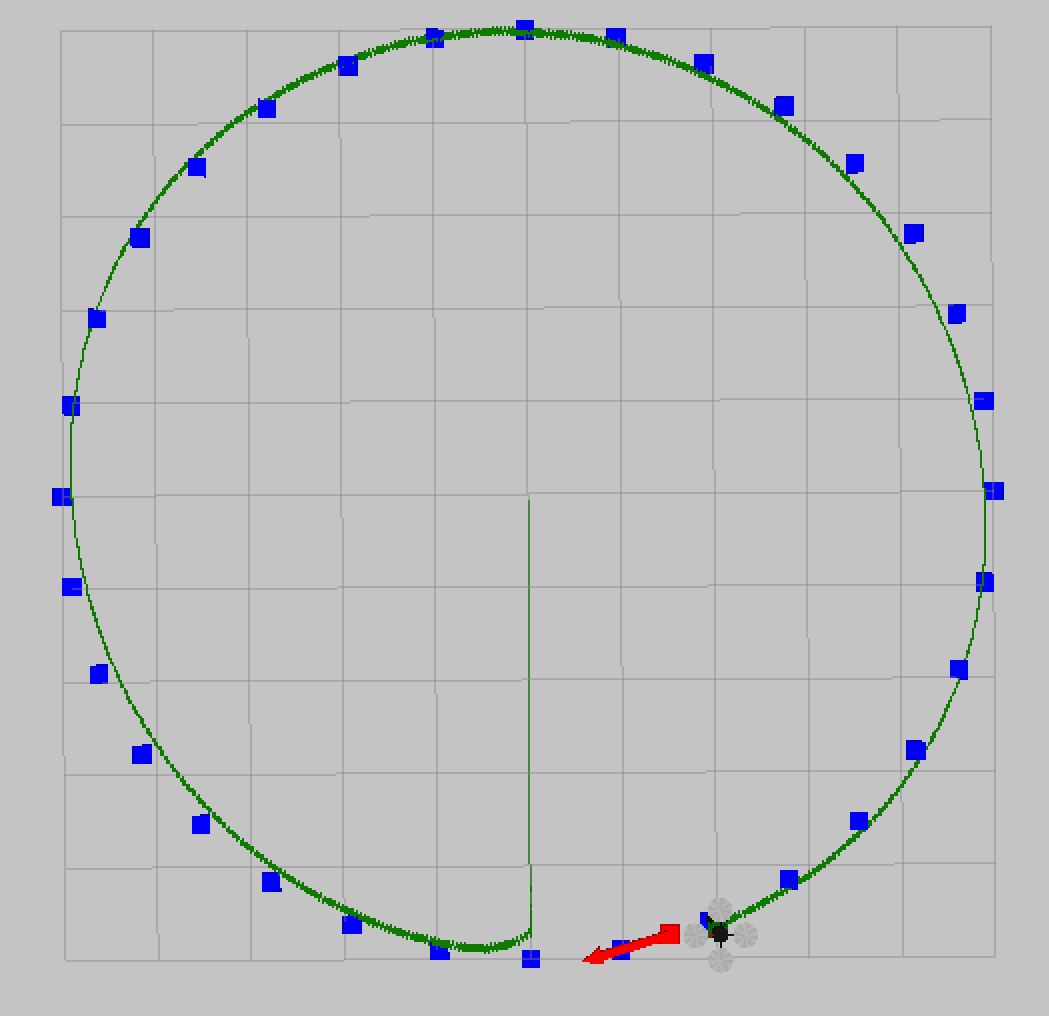
\includegraphics[width=\textwidth]{Pure_Pursuit_0_5_payload_0_25.png}
      \caption{Payload mass=0.25kg, Lookahead=0.5m}
  \end{subfigure}
  \caption{Payload trajectory control using Pure Pursuit.}
\end{figure}
It can be observed that although the trajectory is followed very closely due to the short lookahead distance, a lot of perturbations are introduced due to the motion of the payload relative to the quadrotor. If the weight of the payload is increased further, the oscillations increase drastically.

The actual comparisons can be seen in the speed variation of the 2 cases below.
\begin{figure}[H]
  \centering
  \begin{subfigure}[t]{0.48\textwidth}
    \centering
      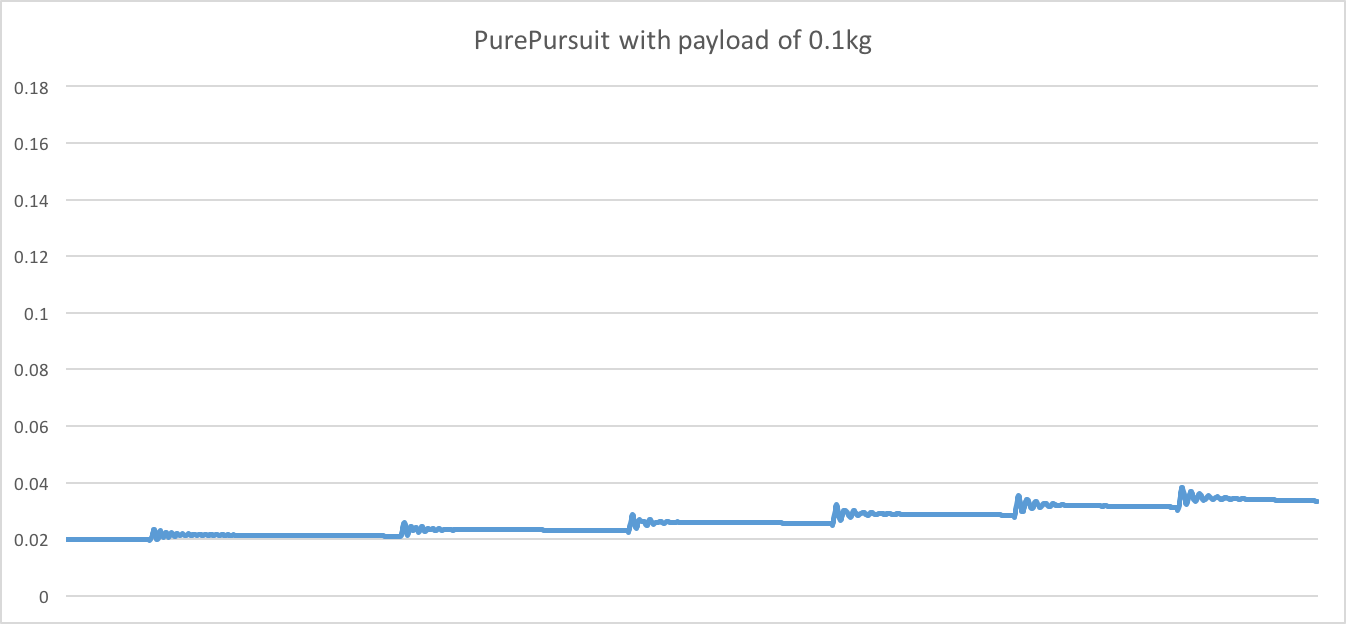
\includegraphics[width=\textwidth]{Pure_Pursuit_speed_payload_0_1.png}
      \caption{Payload mass=0.1	kg}
  \end{subfigure}  \begin{subfigure}[t]{0.48\textwidth}
  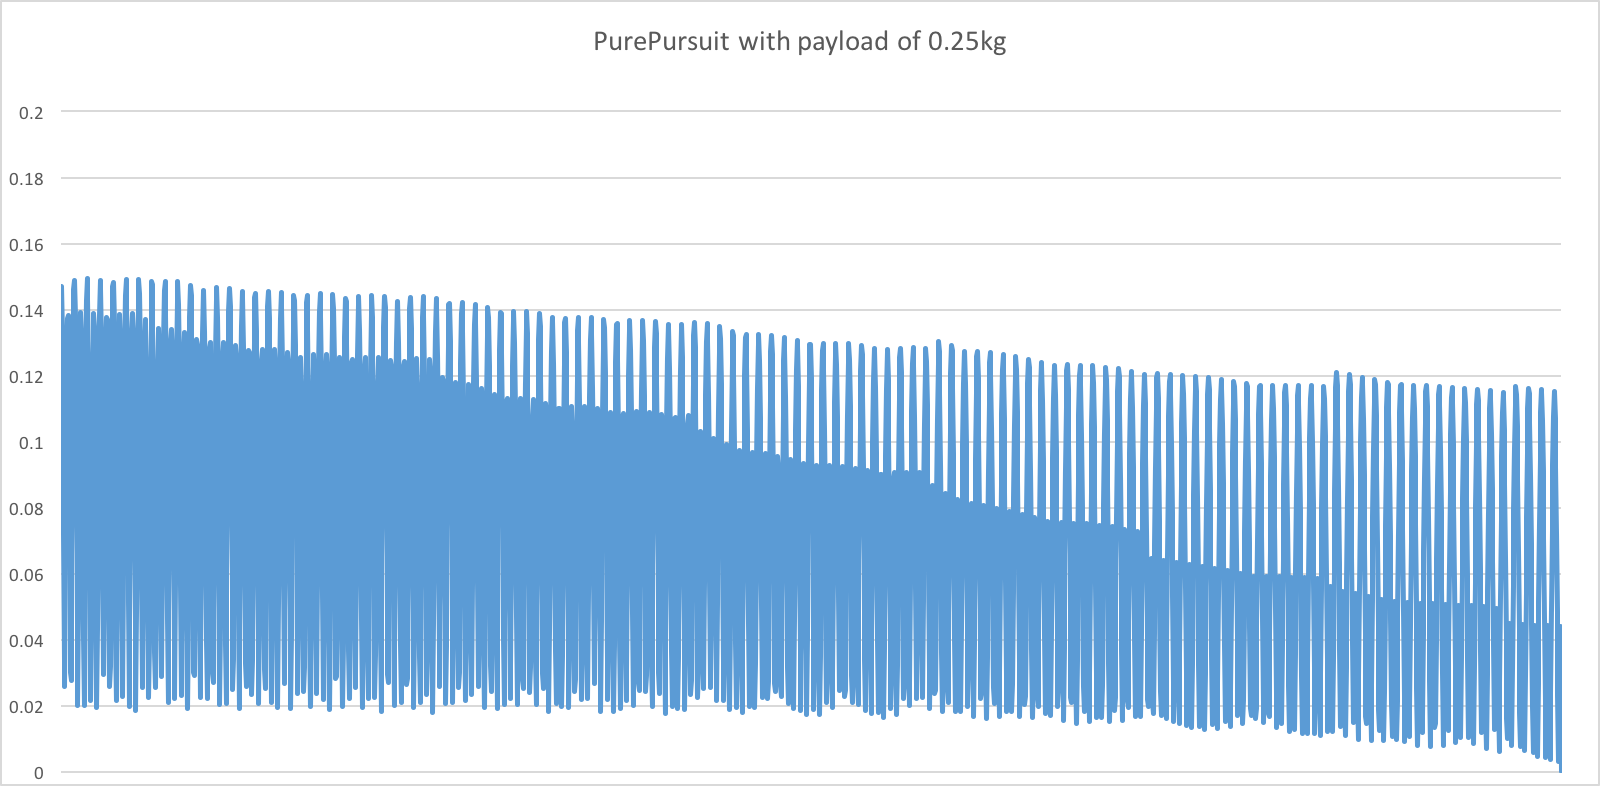
\includegraphics[width=\textwidth]{Pure_Pursuit_speed_payload_0_25.png}
      \caption{Payload mass=0.25kg}
  \end{subfigure}
  \caption{Speed variation in payload trajectory control using Pure Pursuit. Lookahead distance used=0.5m}
\end{figure}	
\subsection*{Effect of wind}
Shorter lookahead distances are much better at countering the wind effect. As seen in the figure, the initial distance from the centre of the circle to the circumference is highly deviated since no trajectory checkpoints are employed here, and simply the controller tries to reach the target. The motion is affected by the wind and the deviation can be reduced by specifying multiple checkpoints. 

Further, it can be noticed that the system with shorter lookahead distance is likely to be easily affected by changes in wind speeds due to lower inertia of motion. Hence, again with respect to stability of the system, a larger lookahead system is preferred.

\begin{figure}[H]
  \centering
  \begin{subfigure}[t]{0.48\textwidth}
    \centering
      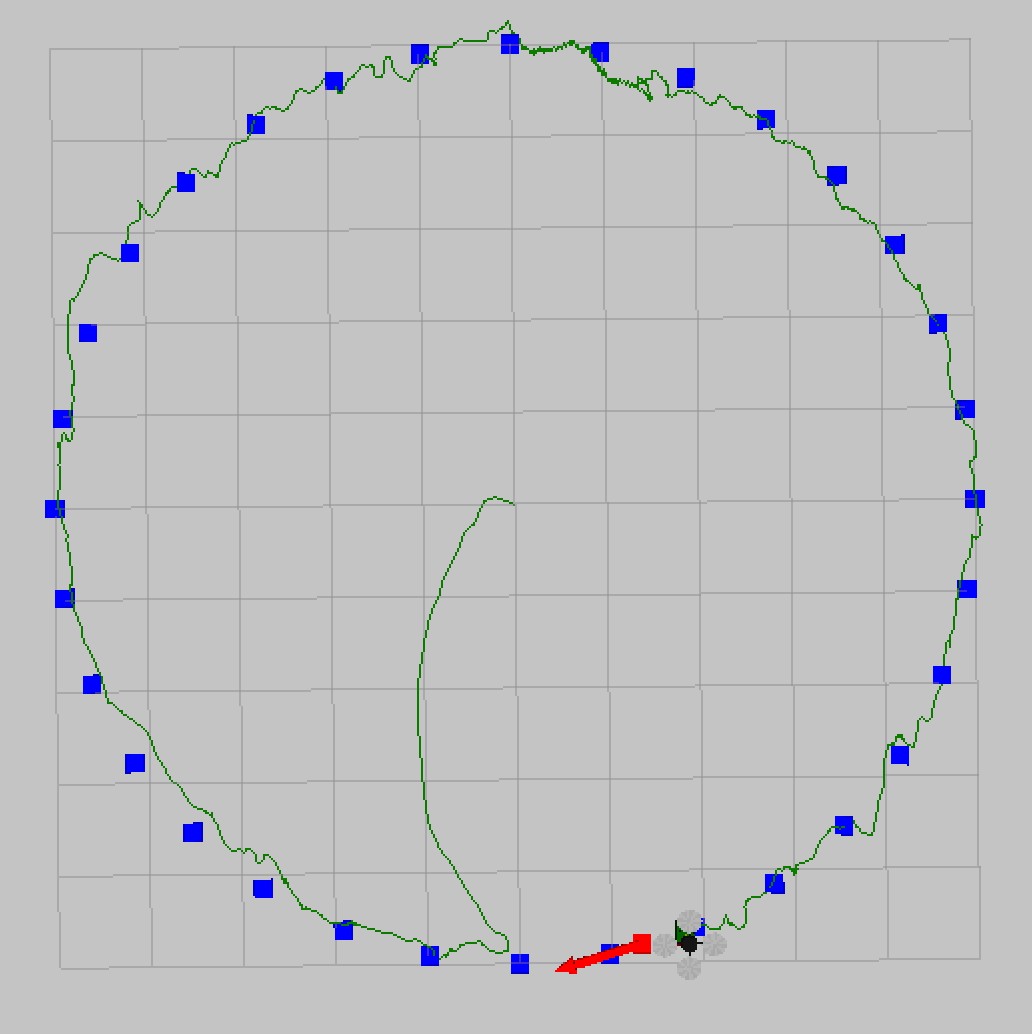
\includegraphics[width=\textwidth]{Pure_Pursuit_0_5_payload_0_1_wind.png}
      \caption{Lookahead distance=0.5m}
  \end{subfigure}  \begin{subfigure}[t]{0.48\textwidth}
  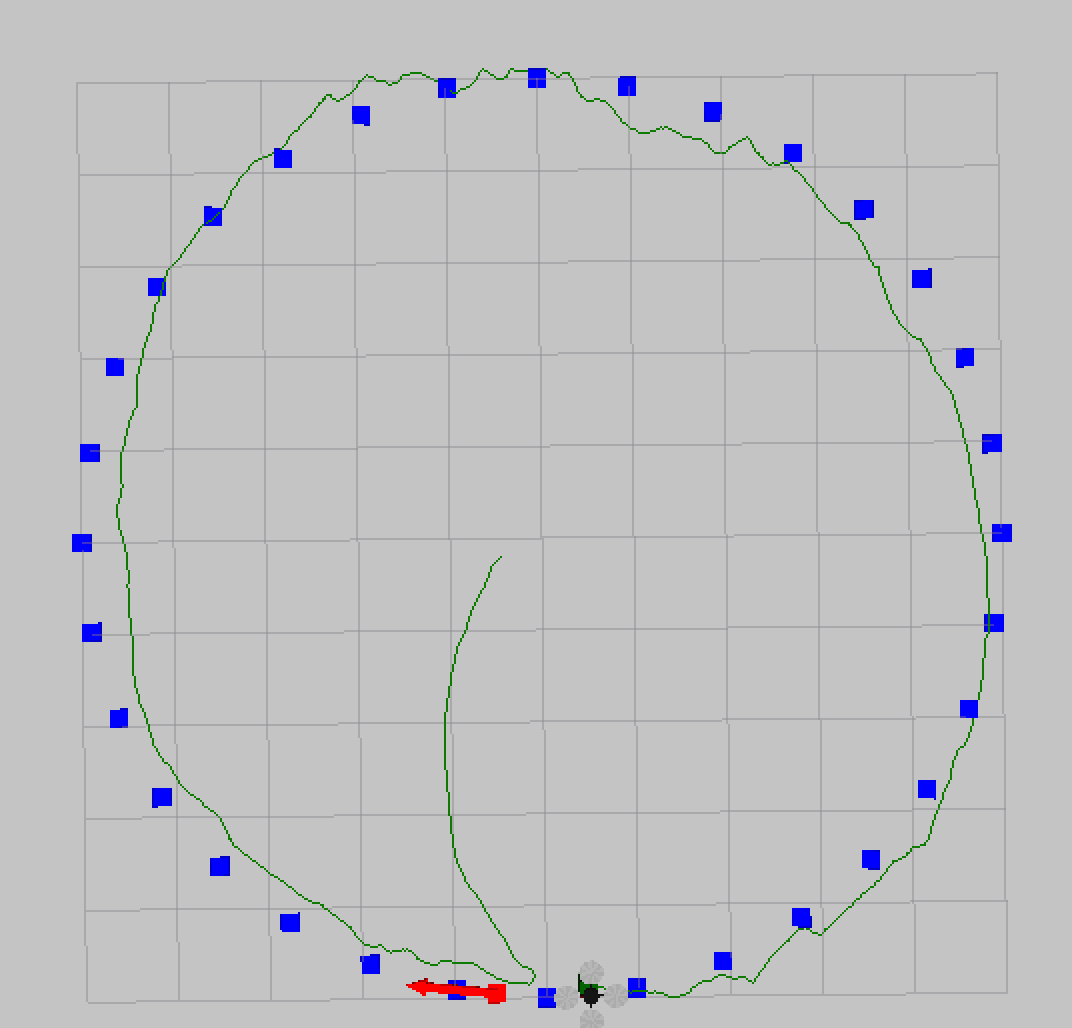
\includegraphics[width=\textwidth]{Pure_Pursuit_1_payload_0_1_wind.png}
      \caption{Lookahead distance=1m}
  \end{subfigure}
  \caption{Payload trajectory control using Pure Pursuit with effect of wind. Both the figures are comparable since identical seeds were used to get the wind.}
\end{figure}	

%%%%%%%%%%%%%%%%%%%%%%%%%%%%%%%%%%%%%%%%%%%%%%%%%%%%%%%%%%%%%%%%%%%%%%%%%%%%%%%%
\chapter{Apprenticeship learning}
We have implemented apprenticeship learning for learning trajectories that are may be complex to be given as a closed form function but can easily be repeatedly done in a close to optimal way using an expert. Additionally, this can be improvised to reach "unstable" states as there is no easy way to define those states using a simple PEGASUS controller. Unstable trajectories comprise of cases such as flips, loops, rolls etc. Apprenticeship based learning involves having an "expert" showing the system how to achieve a certain trajectory. During this the contribution of the "expert" is not to teach the system i.e. it doesn't really give any information to the system. The system is expected to learn by observing the actions of the expert. 
 
 It is assumed that the expert is actually a sub-optimal policy, given the fact that he or she can't repeat his actions exactly multiple times. The job of the system is to use these sub-optimal policies followed by the expert, and use them to find the optimal policy for achieving the motion.

\section{Collecting observations}
The trajectories are sampled using sampling for a number trajectories using a threshold probability of capturing the state information. The state is considered for the trajectory if a random variable sampled from a uniform distribution is greater than the threshold probability. The number of observations considered depends on the complexity of the trajectory, the amount of threshold considered for taking the input data. 
\begin{equation}
	x_P \geq P_t 	
\end{equation}
where $x_P \sim \tilde U\in[0,1]$ and $P_t$ is the threshold probability of considering the state. This is done for the following reasons:
\begin{itemize}
	\item The simulator system is much better than the real world system in prediction of state information. In case of real world environment, uncertainties can lead to a few states being incorrectly measured, or getting false data of the states. So under-sampling the observed trajectories tries to address the issues. 
	\item It is an effort to find the optimal trajectory over the given sub-optimal trajectories. Reducing $P_t$ requires the number of trajectories sampled to increase and the amount of over-fitting on any particular trajectory is bound to decrease. 
	\item It helps to much better mimic the real world scenario for getting/storing data from the system, where the time between two observations will never be the same. There can be further stochasticity in transmission of data, wireless systems can have dropped signals etc.
\end{itemize}


\section{System modelling}
The state for apprenticeship learning is comprised of the absolute position, orientation and velocities of the system:
\begin{equation}
	State[s] = [x,y,z,\omega, \dot x, \dot y, \dot z, \dot \omega]
\end{equation}
The given M demonstrations by an expert are represented by: 
\begin{equation}
y^m = [s^m_1, s^m_2, ..... , s^m_n]	
\end{equation}
where $m \in [1, M]$ is the index of the trajectory and $s$ represents each of the states in the trajectory from time indices 1 to n. The hidden trajectory is given by:
\begin{equation}
	z = [s^*_1, s^*_2, ....... , s^*_T]
\end{equation}
where $T$ represents the length of the hidden trajectory. The hidden model assumes that the demonstrations are a non-linear function of set of observations of the hidden trajectory, i.e.
\begin{equation}
  y_{t}^{k} = h(x_{\tau_t^k}) + {\omega}_{t}^{(y)}, \qquad \omega_t^{(y)} \sim \mathcal{N} (0, \Sigma^{(y)})
\end{equation}
where $\tau_t^k$ is the time step in the intended trajectory mapped to the observed trajectory at time step $t$. These time indices $\tau_t^k$ are not known and need to be found.   

\section{Hidden trajectory}
The hidden trajectory is assumed to be a Markov chain from which the observed trajectory is sampled as explained by the equations above. All the observed trajectories have different time sampling indices due to the stochasticity involved. Hence, we try to combine these various trajectories to estimate the hidden trajectory.

\begin{figure}[H]
  \centering
    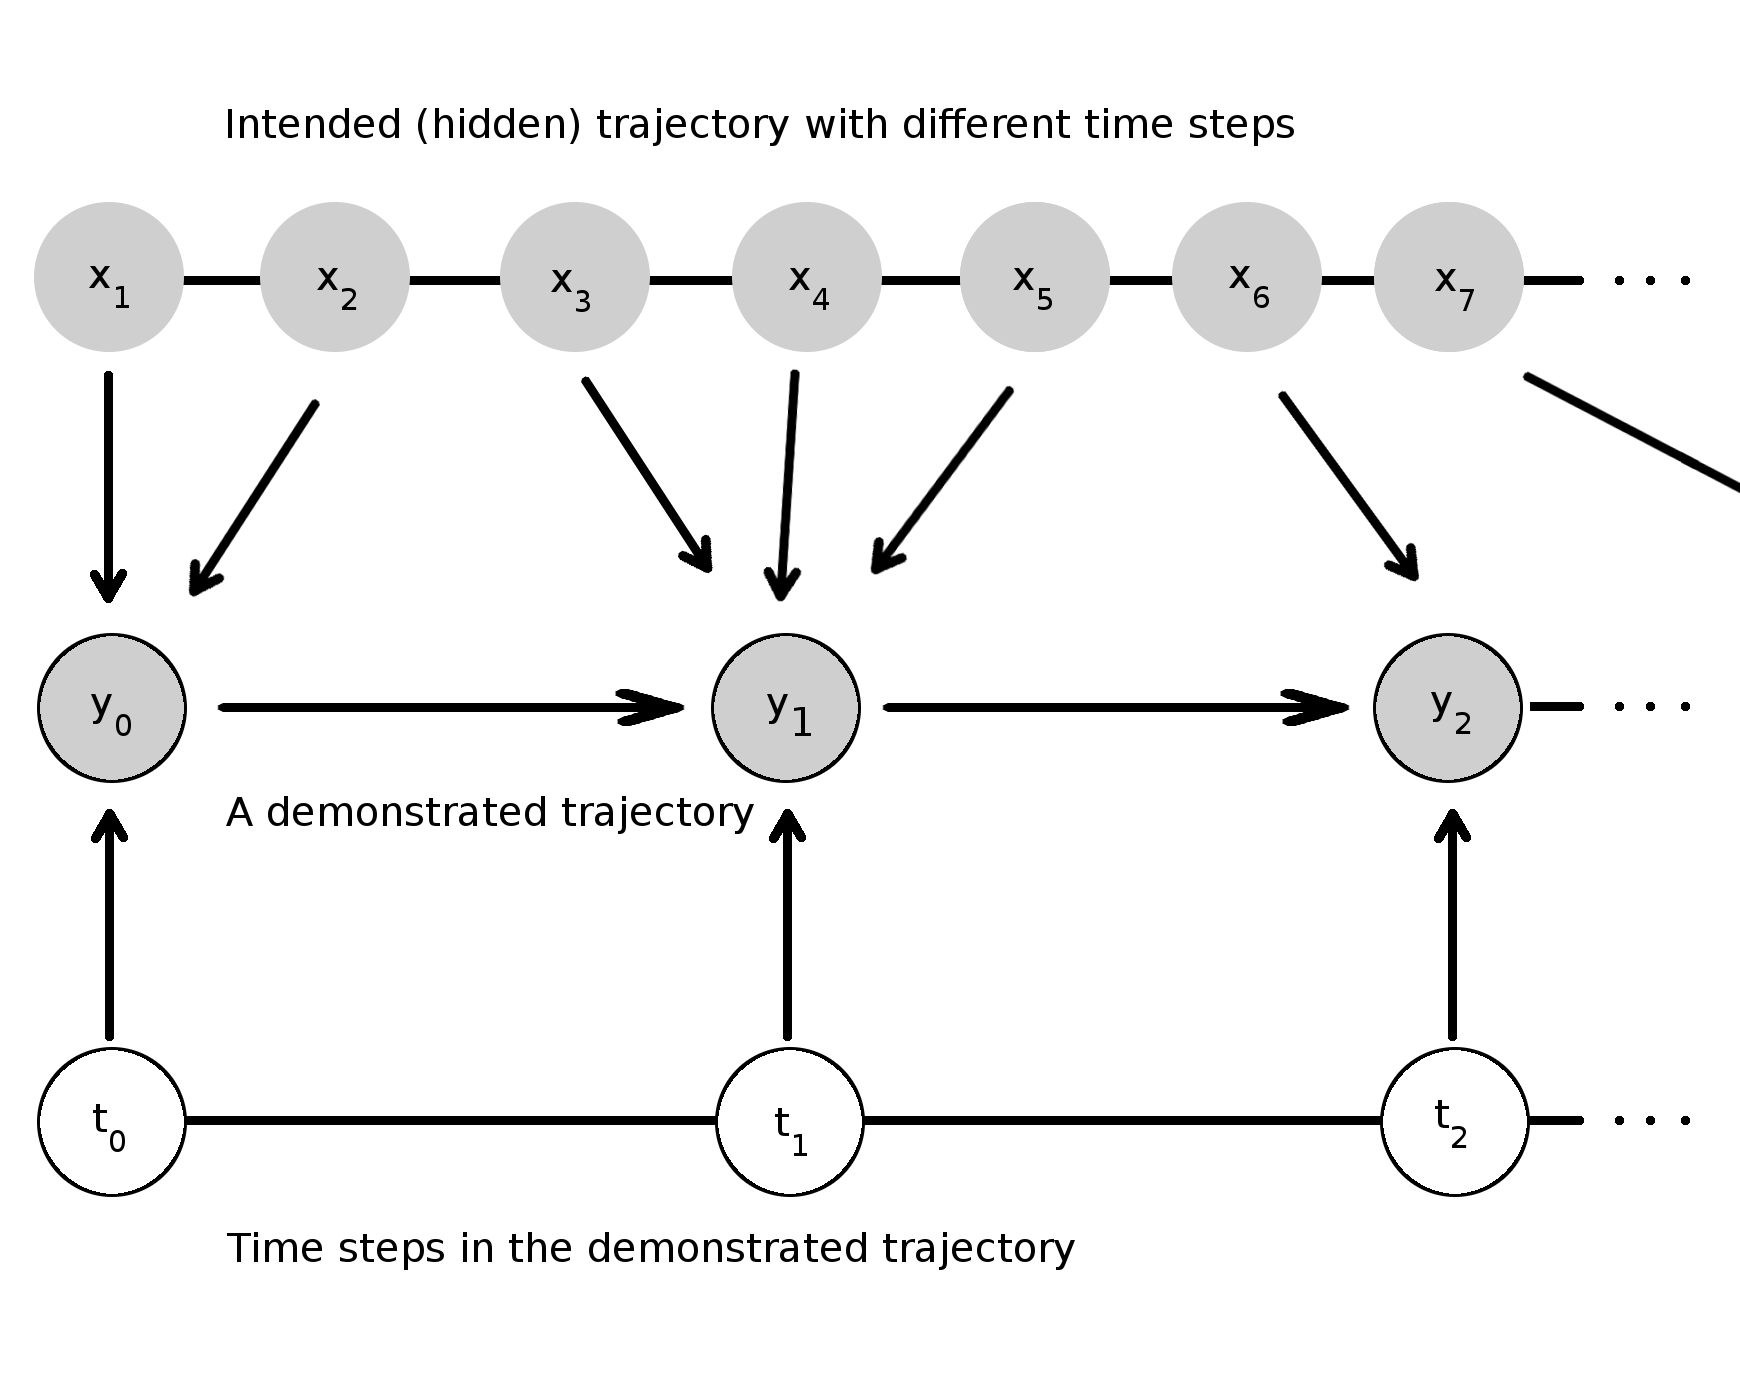
\includegraphics[width=0.7\textwidth]{timewarp.png}
    \caption{Demonstrated trajectory's time warped to align with the time dimension of the intended trajectory.}
\end{figure}

\subsection{Estimating the hidden trajectory}
The estimation of the hidden trajectory can be done by considering the non-linear model of the quadrotor system. The model as explained in the quadrotor dynamics is complicated, and the use of the model challenges the purpose of Reinforcement Learning. 

Our implementation is totally a model-free system, and the estimation step is a mean calculation step for the system. Besides being extremely simple in implementation, it also is very quick computationally, and the results obtained were satisfactory.


\subsection{Dynamic Time warping to calculate the time series of the hidden trajectory}
The different observed trajectories don't have corresponding matching time steps, hence we use dynamic time warping to compare the different sequences of observations spatially. DTW tries to warp time based similar sequences based on their closeness in space. By trial and error, slantedband windowing was the best suited for our use case the best. 

\subsection{Finding the optimal trajectory}
The optimal trajectory is computed by maximizing the joint probability distribution of the observed trajectories and the time indices by marginalizing over the hidden trajectory. This can be represented by:
\begin{equation} 
  \max_{\tau, \Sigma^{(\cdot)}} \log \mathbb{P}(\mathbf{y}, \tau ; \Sigma^{(\cdot)})
\end{equation}
where $\tau$ represents the time indices and $\Sigma^{(\cdot)}$ represents the covariances of the system.

Due to the complexity in computing the above likelihood, the solution is found in an iterative manner using Expectation Maximization. The time series is used as a latent variable for calculating the likelihood, and then DTW is used to re-calculate the time series.

\subsection{Implementation}
The steps followed for estimating the hidden trajectory are given as follows:
\begin{itemize}
	\item Assume the number of time indices to consider as the hidden trajectory's length. We have used the hidden trajectory length as $2*(average(length-of-observed-trajectory))$.
	\item Our implementation just has the state vector as representation of the trajectory due to the fact that our PEGASUS based controller is capable of reaching a certain state. In the absence of such a controller, both the states and actions can be included as part of both the observations and the hidden trajectory.
	\item An initial assumption is considered for the time indices of each of the observed trajectories. The hidden trajectory is calculated from these observed trajectories then. The hidden trajectory is calculated as the average of the states at a current time step. This gives an initial estimate for the hidden trajectory. In EM terms, this is the Estimation step.
	\item Each of the observed trajectories is used to apply a DTW warping with hidden trajectory to estimate the time indices for the observed trajectories. This represents the Maximization step.
	\item The above two steps are repeated until a stable hidden trajectory is found from the observed trajectories.
	\item Finally the states from the hidden trajectory are used to run the quadrotor system.
\end{itemize}

\section{Controlling using trajectory}
The system predicts the next $s'$ that the quadrotor needs to be in given the current $s$. The mapping for the predictor is from $S: \rightarrow S$. To follow the trajectory in a perfectly optimal fashion, a controller such as Differential Dynamic Programming controller can be used as the state and action information between two given states can be predicted in that case.

We have implemented the original PEGASUS controller with trajectory control methods, due to its capability of going to the final state $s'$ from the original state. The trajectory tracking sequence ensures that the quadrotor is on the correct trajectory. This has given satisfactory results with the system.

\section{Results}
The results here represent circle trajectory sampled using 6 trajectories with probability of data collection as 0.5. The system considered is quadrotor with payload of 0.1kg. The wind in these trajectories is continuously changing leading to small to large variations in the trajectory followed and the stability of the quadrotor-payload system. 

\begin{figure}[H]
  \centering
    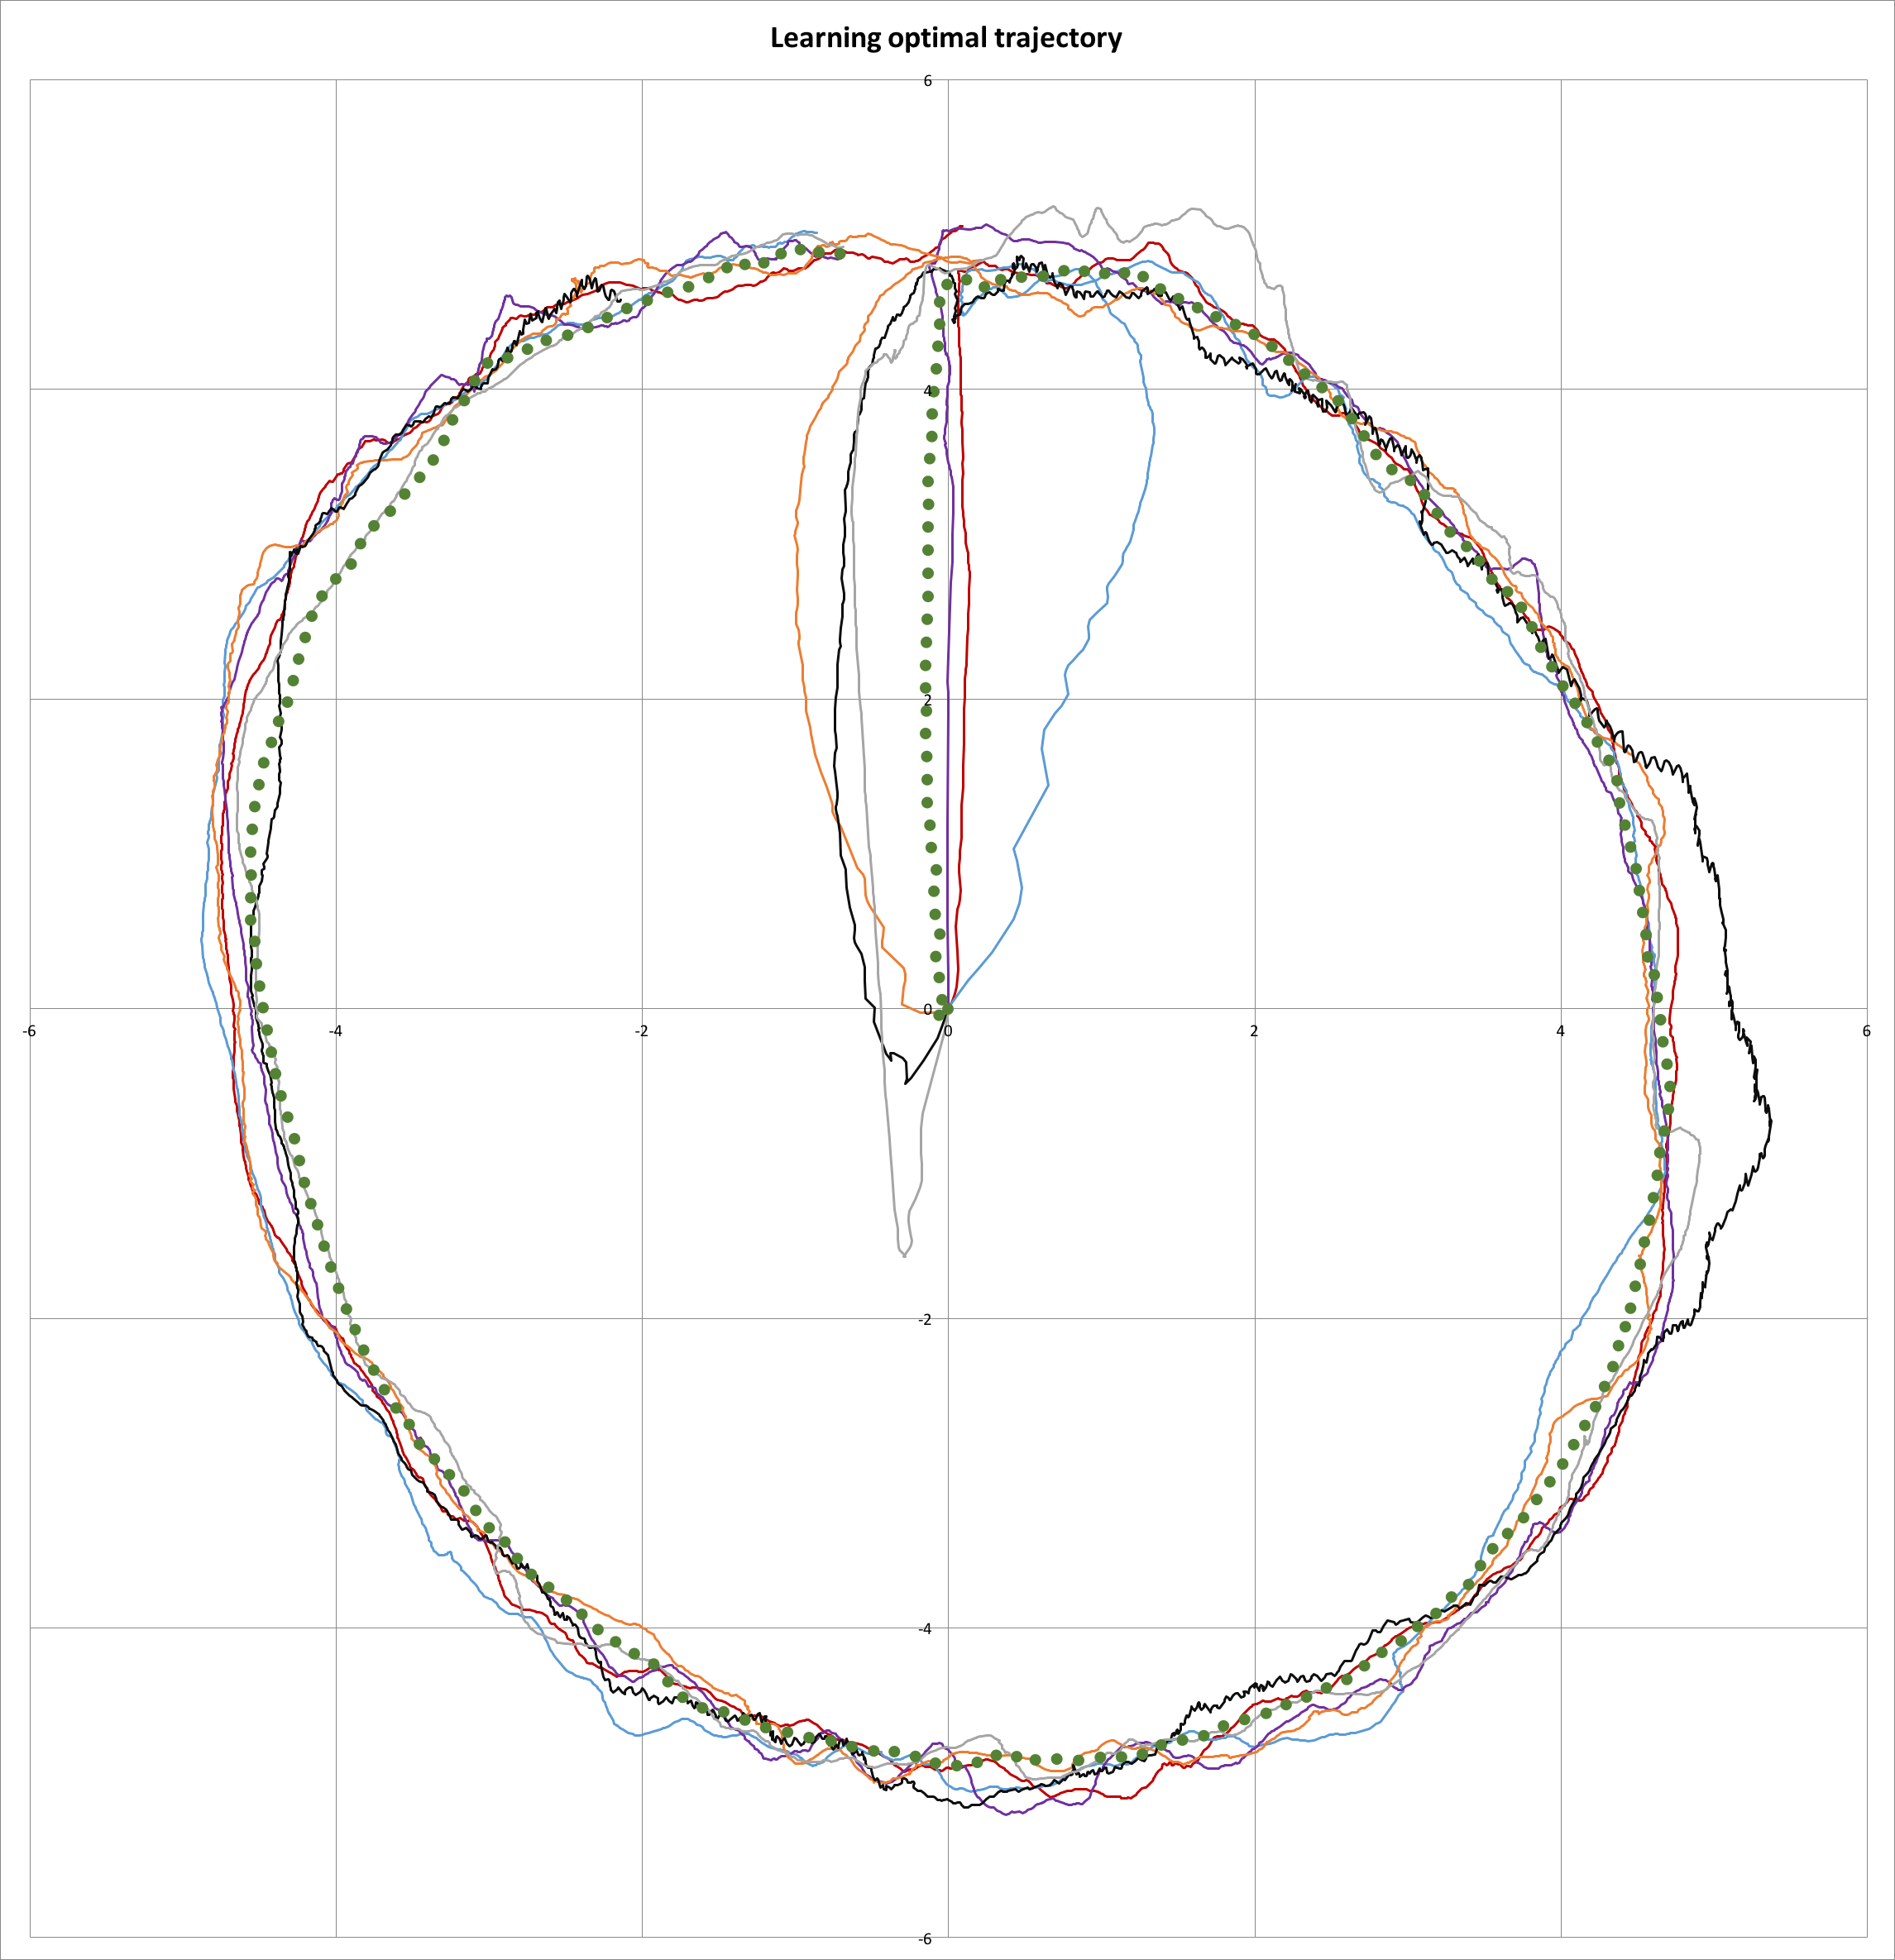
\includegraphics[width=\textwidth]{Apprenticeship_hidden_trajectory.png}
    \caption{Hidden trajectory found using observations for a circular trajectory.The dotted trajectory represents the learnt trajectory.}
\end{figure}

The optimality of the hidden trajectory can be observed by finding the circularity error ie $radius^2 - (x-x_0)^2 - (y-y_0)^2$. In all the cases, the average error is close to the observed average error.
\begin{figure}[H]
  \centering
    \includegraphics[width=0.7\textwidth]{Apprenticeship_optimality_graph.png}
    \caption{Average circle error for observed and hidden trajectories.}
\end{figure}	

The control using the hidden trajectory, as expected from the average error graph, is pretty stable. The trajectory controller used was Pure Pursuit controller with a lookahead distance of 0.5m. In the stochastic case involving wind in the system, the trajectory is affected, but due to the smooth trajectory and the Pure Pursuit controller, most of these vibrations are curbed.
\begin{figure}[H]
  \centering
  \begin{subfigure}[t]{0.48\textwidth}
  \includegraphics[width=\textwidth]{Apprenticeship_Pure_Pursuit_0_5_payload_0_1.png}
      \caption{No wind}
  \end{subfigure}
  \begin{subfigure}[t]{0.48\textwidth}
    \centering
      \includegraphics[width=\textwidth]{Apprenticeship_Pure_Pursuit_0_5_payload_0_1_wind_5.png}
      \caption{With wind}
  \end{subfigure}
  \caption{Using trajectory learnt using sampled observations to control motion of quadrotor.}
\end{figure}
Further we report the results with Dynamic time warping the observed series with respect to the hidden trajectory. Using a very large band, the results are wrong.
\begin{figure}[H]
  \centering
    \includegraphics[width=0.6\textwidth]{DTW_no_band.png}
    \caption{Using a large band for DTW, although the mapping is mathematically optimal, yet incorrect.}
\end{figure}	
Narrowing down the band gives a correct trajectory estimate which is similar to the actual expected estimate given the knowledge of the observations. The figure represents DTW iterations of a single observation with the hidden trajectory till the optimal mapping is found.
\begin{figure}[H]
  \centering
  \begin{subfigure}[t]{0.48\textwidth}
  \includegraphics[width=\textwidth]{DTW_with_band_iter_1.png}
      \caption{First iteration}
  \end{subfigure}
  \begin{subfigure}[t]{0.48\textwidth}
    \centering
      \includegraphics[width=\textwidth]{DTW_with_band_iter_final.png}
      \caption{Final iteration}
  \end{subfigure}
  \caption{DTW iterations using slate band windowing method. The initial trajectory is closer to the window and finally the optimal mappings are found.}
\end{figure}

\chapter{Conclusions and Future scope}
We have shown optimal control on a quadrotor to achieve a desired position, and have used it in trajectory tracking algorithms to achieve the trajectories with accuracy and stability as the target. Our controller is based on PEGASUS, and can be simply be used for any other multi-rotor, since there is no dependence on the quadrotor model, or the number of motors. The trajectory tracking algorithm Pure Pursuit helps achieve both a stable and accurate trajectory.

There are some future ideas to continue on this project:
\begin{itemize}
	\item The simulator has opened a possibility of exploring various reinforcement learning algorithms in the field of quadrotor control. It would be interesting to work on different problems in the quadrotor domain such as employing Predator-Prey methods in swarm based robotics, or using Deep Neural networks to find the optimal control policy class. 
	\item The Pure Pursuit algorithm has the issues of having a constant lookahead, and having a variable lookahead which is learnt using a Reinforcement Learning task would be an interesting idea. The feature for the same would depend on the trajectory.
	\item The Apprenticeship based learning method currently learns only simple trajectories. By adding support for unstable states in the simulator, the method can be extended to harder problems involving unstable trajectories such as flips which would be a suitable implementation for the Apprenticeship learning setup.
\end{itemize}

%%%%%%%%%%%%%%%%%%%%%%%%%%%%%%%%%%%%%%%%%%%%%%%%%%%%%%%%%%%%
% Bibliography.

\begin{singlespace}
  \pagebreak
  \clearpage
  \phantomsection
  \addcontentsline{toc}{chapter}{References}
  \bibliography{refs}
\end{singlespace}

\end{document}
